
%%%%%%%%%%%%%%%%%%%%%%%%%%%%%%%%%%%%%%%%%%%%%%%%%%%%%%%%%%%%%%%%%%%%%%%%
%     Preamble                                                         %
%%%%%%%%%%%%%%%%%%%%%%%%%%%%%%%%%%%%%%%%%%%%%%%%%%%%%%%%%%%%%%%%%%%%%%%%

% ----------------------------------------------------------------------
%  Set the document class
% ----------------------------------------------------------------------
\documentclass[10pt,a4paper,twoside]{report}

% ----------------------------------------------------------------------
% Define external packages, language, margins, fonts and new commands
% ----------------------------------------------------------------------
%%%%%%%%%%%%%%%%%%%%%%%%%%%%%%%%%%%%%%%%%%%%%%%%%%%%%%%%%%%%%%%%%%%%%%%%
%                                                                      %
%     File: Thesis_Preamble.tex                                        %
%     Tex Master: Thesis.tex                                           %
%                                                                      %
%     Author: ENES UYSAL                                           %
%     Last modified : 9 Apr 2015                                       %
%                                                                      %
%%%%%%%%%%%%%%%%%%%%%%%%%%%%%%%%%%%%%%%%%%%%%%%%%%%%%%%%%%%%%%%%%%%%%%%%

% ----------------------------------------------------------------------
% Define document language.
% ----------------------------------------------------------------------

% 'inputenc' package
%
% Accept different input encodings.
% http://www.ctan.org/tex-archive/macros/latex/base/
%
% > allows typing non-english text in LaTeX sources.
%
% ******************************* SELECT *******************************
%\usepackage[latin1]{inputenc} % <<<<< Windows
\usepackage[utf8]{inputenc}   % <<<<< Linux
% ******************************* SELECT *******************************


% 'babel' package
%
% Multilingual support for Plain TeX or LaTeX.
% http://www.ctan.org/tex-archive/macros/latex/required/babel/
%
% > sets the variable names according to the language selected
%
% ******************************* SELECT *******************************
%\usepackage[portuguese]{babel} % <<<<< Portuguese
\usepackage[english]{babel} % <<<<< English
% ******************************* SELECT *******************************


% List of LaTeX variable names: \abstractname, \appendixname, \bibname,
%   \chaptername, \contentsname, \listfigurename, \listtablename, ...)
% http://www.tex.ac.uk/cgi-bin/texfaq2html?label=fixnam
%
% Changing the words babel uses (uncomment and redefine as necessary...)
%
\newcommand{\acknowledgments}{@undefined} % new LaTeX variable name
%
% > English
%
\addto\captionsenglish{\renewcommand{\acknowledgments}{Acknowledgments}}
%\addto\captionsenglish{\renewcommand{\contentsname}{Contents}}
%\addto\captionsenglish{\renewcommand{\listtablename}{List of Tables}}
%\addto\captionsenglish{\renewcommand{\listfigurename}{List of Figures}}
%\addto\captionsenglish{\renewcommand{\nomname}{Nomenclature}}
%\addto\captionsenglish{\renewcommand{\glossaryname}{Glossary}}
%\addto\captionsenglish{\renewcommand{\acronymname}{List of Acronyms}}
%\addto\captionsenglish{\renewcommand{\bibname}{References}} % Bibliography
%\addto\captionsenglish{\renewcommand{\appendixname}{Appendix}}

% > Portuguese
%
\addto\captionsportuguese{\renewcommand{\acknowledgments}{Agradecimentos}}
%\addto\captionsportuguese{\renewcommand{\contentsname}{Conte\'{u}do}}
%\addto\captionsportuguese{\renewcommand{\listtablename}{Lista de Figuras}}
%\addto\captionsportuguese{\renewcommand{\listfigurename}{Lista de Tabelas}}
\addto\captionsportuguese{\renewcommand{\nomname}{Lista de S\'{i}mbolos}} % Nomenclatura
%\addto\captionsportuguese{\renewcommand{\glossary}{Gloss\'{a}rio}}
%\addto\captionsportuguese{\renewcommand{\acronymname}{Lista de Abrevia\c{c}\~{o}es}}
%\addto\captionsportuguese{\renewcommand{\bibname}{Refer\^{e}ncias}} % Bibliografia
%\addto\captionsportuguese{\renewcommand{\appendixname}{Anexo}} % Apendice


% ----------------------------------------------------------------------
% Define cover fields in both english and portuguese.
% ----------------------------------------------------------------------
%
\newcommand{\coverThesis}{@undefined} % new LaTeX variable name
\newcommand{\coverSupervisors}{@undefined} % new LaTeX variable name
\newcommand{\coverExaminationCommittee}{@undefined} % new LaTeX variable name
\newcommand{\coverChairperson}{@undefined} % new LaTeX variable name
\newcommand{\coverSupervisor}{@undefined} % new LaTeX variable name
\newcommand{\coverMemberCommittee}{@undefined} % new LaTeX variable name
% > English
\addto\captionsenglish{\renewcommand{\coverThesis}{Thesis to obtain the Master of Science Degree in}}
\addto\captionsenglish{\renewcommand{\coverSupervisors}{Supervisor(s)}}
\addto\captionsenglish{\renewcommand{\coverExaminationCommittee}{Examination Committee}}
\addto\captionsenglish{\renewcommand{\coverChairperson}{Chairperson}}
\addto\captionsenglish{\renewcommand{\coverSupervisor}{Supervisor}}
\addto\captionsenglish{\renewcommand{\coverMemberCommittee}{Member of the Committee}}
% > Portuguese
\addto\captionsportuguese{\renewcommand{\coverThesis}{Disserta\c{c}\~{a}o para obten\c{c}\~{a}o do Grau de Mestre em}}
\addto\captionsportuguese{\renewcommand{\coverSupervisors}{Orientador(es)}}
\addto\captionsportuguese{\renewcommand{\coverExaminationCommittee}{J\'{u}ri}}
\addto\captionsportuguese{\renewcommand{\coverChairperson}{Presidente}}
\addto\captionsportuguese{\renewcommand{\coverSupervisor}{Orientador}}
\addto\captionsportuguese{\renewcommand{\coverMemberCommittee}{Vogal}}


% ----------------------------------------------------------------------
% Define default and cover page fonts.
% ----------------------------------------------------------------------

% Use Arial font as default
%
\renewcommand{\rmdefault}{phv}
\renewcommand{\sfdefault}{phv}

% Define cover page fonts
%
%         encoding     family       series      shape
%  \usefont{T1}     {phv}=helvetica  {b}=bold    {n}=normal
%                   {ptm}=times      {m}=normal  {sl}=slanted
%                                                {it}=italic
% see more examples at
% http://julien.coron.free.fr/languages/latex/fonts/
%
\def\FontLn{% 16 pt normal
  \usefont{T1}{phv}{m}{n}\fontsize{16pt}{16pt}\selectfont}
\def\FontLb{% 16 pt bold
  \usefont{T1}{phv}{b}{n}\fontsize{16pt}{16pt}\selectfont}
\def\FontMn{% 14 pt normal
  \usefont{T1}{phv}{m}{n}\fontsize{14pt}{14pt}\selectfont}
\def\FontMb{% 14 pt bold
  \usefont{T1}{phv}{b}{n}\fontsize{14pt}{14pt}\selectfont}
\def\FontSn{% 12 pt normal
  \usefont{T1}{phv}{m}{n}\fontsize{12pt}{12pt}\selectfont}


% ----------------------------------------------------------------------
% Define page margins and line spacing.
% ----------------------------------------------------------------------

% 'geometry' package
%
% Flexible and complete interface to document dimensions.
% http://www.ctan.org/tex-archive/macros/latex/contrib/geometry/
%
% > set the page margins (2.5cm minimum in every side, as per IST rules)
%
\usepackage{geometry}
\geometry{verbose,tmargin=2.5cm,bmargin=2.5cm,lmargin=2.5cm,rmargin=2.5cm}

% 'setspace' package
%
% Set space between lines.
% http://www.ctan.org/tex-archive/macros/latex/contrib/setspace/
%
% > allow setting line spacing (line spacing of 1.5, as per IST rules)
%
\usepackage{setspace}
\renewcommand{\baselinestretch}{1.5}


% ----------------------------------------------------------------------
% Include external packages.
% Note that not all of these packages may be available on all system
% installations. If necessary, include the .sty files locally in
% the <jobname>.tex file directory.
% ----------------------------------------------------------------------

% 'graphicx' package
%
% Enhanced support for graphics.
% http://www.ctan.org/tex-archive/macros/latex/required/graphics/
%
% > extends arguments of the \includegraphics command
%
\usepackage{graphicx}


% 'color' package
%
% Colour control for LaTeX documents.
% http://www.ctan.org/tex-archive/macros/latex/required/graphics/
%
% > defines color macros: \color{<color name>}
%
%\usepackage{color}


% 'amsmath' package
%
% Mathematical enhancements for LaTeX.
% http://www.ctan.org/tex-archive/macros/latex/required/amslatex/
%
% > American Mathematical Society plain Tex macros
%
\usepackage{amsmath}  % AMS mathematical facilities for LaTeX.
\usepackage{amsthm}   % Typesetting theorems (AMS style).
\usepackage{amsfonts} %


% 'wrapfig' package
%
% Produces figures which text can flow around.
% http://www.ctan.org/tex-archive/macros/latex/contrib/wrapfig/
%
% > wrap figures/tables in text (i.e., Di Vinci style)
%
% \usepackage{wrapfig}


% 'subfigure' package
%
% Deprecated: Figures divided into subfigures.
% http://www.ctan.org/tex-archive/obsolete/macros/latex/contrib/subfigure/
%
% > subcaptions for subfigures
%
\usepackage{subfigure}


% 'subfigmat' package
%
% Automates layout when using the subfigure package.
% http://www.ctan.org/tex-archive/macros/latex/contrib/subfigmat/
%
% > matrices of similar subfigures
%
\usepackage{subfigmat}


% 'url' package
%
% Verbatim with URL-sensitive line breaks.
% http://www.ctan.org/tex-archive/macros/latex/contrib/url/
%
% > URLs in BibTex
%
% \usepackage{url}


% 'varioref' package
%
% Intelligent page references.
% http://www.ctan.org/tex-archive/macros/latex/required/tools/
%
% > smart page, figure, table and equation referencing
%
%\usepackage{varioref}


% 'dcolumn' package
%
% Align on the decimal point of numbers in tabular columns.
% http://www.ctan.org/tex-archive/macros/latex/required/tools/
%
% > decimal-aligned tabular math columns
%
\usepackage{dcolumn}
\newcolumntype{d}{D{.}{.}{-1}} % column aligned by the point separator '.'
\newcolumntype{e}{D{E}{E}{-1}} % column aligned by the exponent 'E'


% '' package
%
% Reimplementation of and extensions to LaTeX verbatim.
% http://www.ctan.org/tex-archive/macros/latex/required/tools/
%
% > provides the verbatim environment (\begin{verbatim},\end{verbatim})
%   and a comment environment (\begin{comment},  \end{comment})
%
% \usepackage{verbatim}


% 'moreverb' package
%
% Extended verbatim.
% http://www.ctan.org/tex-archive/macros/latex/contrib/moreverb/
%
% > supports tab expansion and line numbering
%
% \usepackage{moreverb}



% 'nomencl' package
%
% Produce lists of symbols as in nomenclature.
% http://www.ctan.org/tex-archive/macros/latex/contrib/nomencl/
%
% The nomencl package makes use of the MakeIndex program
% in order to produce the nomenclature list.
%
% Nomenclature
% 1) On running the file through LATEX, the command \makenomenclature
%    in the preamble instructs it to create/open the nomenclature file
%    <jobname>.nlo corresponding to the LATEX file <jobname>.tex and
%    writes the information from the \nomenclature commands to this file.
% 2) The next step is to invoke MakeIndex in order to produce the
%    <jobname>.nls file. This can be achieved by making use of the
%    command: makeindex <jobname>.nlo -s nomencl.ist -o <jobname>.nls
% 3) The last step is to invoke LATEX on the <jobname>.tex file once
%    more. There, the \printnomenclature in the document will input the
%    <jobname>.nls file and process it according to the given options.
%
% http://www-h.eng.cam.ac.uk/help/tpl/textprocessing/nomencl.pdf
%
% Nomenclature (produces *.nlo *.nls files)
\usepackage{nomencl}
\makenomenclature
%
% Group variables according to their symbol type
%
\RequirePackage{ifthen}
\ifthenelse{\equal{\languagename}{english}}%
    { % English
    \renewcommand{\nomgroup}[1]{%
      \ifthenelse{\equal{#1}{R}}{%
        \item[\textbf{Roman symbols}]}{%
        \ifthenelse{\equal{#1}{G}}{%
          \item[\textbf{Greek symbols}]}{%
          \ifthenelse{\equal{#1}{S}}{%
            \item[\textbf{Subscripts}]}{%
            \ifthenelse{\equal{#1}{T}}{%
              \item[\textbf{Superscripts}]}{}}}}}%
    }{% Portuguese
    \renewcommand{\nomgroup}[1]{%
      \ifthenelse{\equal{#1}{R}}{%
        \item[\textbf{Simbolos romanos}]}{%
        \ifthenelse{\equal{#1}{G}}{%
          \item[\textbf{Simbolos gregos}]}{%
          \ifthenelse{\equal{#1}{S}}{%
            \item[\textbf{Subscritos}]}{%
            \ifthenelse{\equal{#1}{T}}{%
              \item[\textbf{Sobrescritos}]}{}}}}}%
    }%


% 'glossary' package
%
% Create a glossary.
% http://www.ctan.org/tex-archive/macros/latex/contrib/glossary/
%
% Glossary (produces *.glo *.ist files)
\usepackage[number=none]{glossary}
% (remove blank line between groups)
\setglossary{gloskip={}}
% (redefine glossary style file)
%\renewcommand{\istfilename}{myGlossaryStyle.ist}
\makeglossary


% 'rotating' package
%
% Rotation tools, including rotated full-page floats.
% http://www.ctan.org/tex-archive/macros/latex/contrib/rotating/
%
% > show wide figures and tables in landscape format:
%   use \begin{sidewaystable} and \begin{sidewaysfigure}
%   instead of 'table' and 'figure', respectively.
%
\usepackage{rotating}


% 'hyperref' package
%
% Extensive support for hypertext in LaTeX.
% http://www.ctan.org/tex-archive/macros/latex/contrib/hyperref/
%
% > Extends the functionality of all the LATEX cross-referencing
%   commands (including the table of contents, bibliographies etc) to
%   produce \special commands which a driver can turn into hypertext
%   links; Also provides new commands to allow the user to write adhoc
%   hypertext links, including those to external documents and URLs.
%
\usepackage[pdftex]{hyperref} % enhance documents that are to be
                              % output as HTML and PDF
\hypersetup{colorlinks,       % color text of links and anchors,
                              % eliminates borders around links
%            linkcolor=red,    % color for normal internal links
            linkcolor=black,  % color for normal internal links
            anchorcolor=black,% color for anchor text
%            citecolor=green,  % color for bibliographical citations
            citecolor=black,  % color for bibliographical citations
%            filecolor=magenta,% color for URLs which open local files
            filecolor=black,  % color for URLs which open local files
%            menucolor=red,    % color for Acrobat menu items
            menucolor=black,  % color for Acrobat menu items
%            pagecolor=red,    % color for links to other pages
            pagecolor=black,  % color for links to other pages
%            urlcolor=cyan,    % color for linked URLs
            urlcolor=black,   % color for linked URLs
	          bookmarks=true,         % create PDF bookmarks
	          bookmarksopen=false,    % don't expand bookmarks
	          bookmarksnumbered=true, % number bookmarks
	          pdftitle={Thesis},
            pdfauthor={Andre C. Marta},
            pdfsubject={Thesis Title},
            pdfkeywords={Thesis Keywords},
            pdfstartview=FitV,
            pdfdisplaydoctitle=true}


% 'hypcap' package
%
% Adjusting the anchors of captions.
% http://www.ctan.org/tex-archive/macros/latex/contrib/oberdiek/
%
% > fixes the problem with hyperref, that links to floats points
%   below the caption and not at the beginning of the float.
%
\usepackage[figure,table]{hypcap}


% 'natbib' package
%
% Flexible bibliography support.
% http://www.ctan.org/tex-archive/macros/latex/contrib/natbib/
%
% > produce author-year style citations
%
% \citet  and \citep  for textual and parenthetical citations, respectively
% \citet* and \citep* that print the full author list, and not just the abbreviated one
% \citealt is the same as \citet but without parentheses. Similarly, \citealp is \citep without parentheses
% \citeauthor
% \citeyear
% \citeyearpar
%
% ******************************* SELECT *******************************
%\usepackage{natbib}          % <<<<< References in alphabetical list Correia, Silva, ...
\usepackage[numbers]{natbib} % <<<<< References in numbered list [1],[2],...
% ******************************* SELECT *******************************


% 'notoccite' package
%
% Prevent trouble from citations in table of contents, etc.
% http://ctan.org/pkg/notoccite
%
% > If you have \cite com­mands in \sec­tion-like com­mands, or in \cap­tion,
%   the ci­ta­tion will also ap­pear in the ta­ble of con­tents, or list of what­ever.
%   If you are also us­ing an un­srt-like bib­li­og­ra­phy style, these ci­ta­tions will
%   come at the very start of the bib­li­og­ra­phy, which is con­fus­ing. This pack­age
%   sup­presses the ef­fect.
%
\usepackage{notoccite}


% 'multirow' package
%
% Create tabular cells spanning multiple rows
% http://www.ctan.org/pkg/multirow
%
\usepackage{multirow}


% 'booktabs' package
%
% Publication quality tables in LaTeX
% http://www.ctan.org/pkg/booktabs
%
% > en­hance the qual­ity of ta­bles in LaTeX, pro­vid­ing ex­tra com­mands.
%
% \renewcommand{\arraystretch}{<ratio>} % space between rows
%
\usepackage{booktabs}
%\newcommand{\ra}[1]{\renewcommand{\arraystretch}{#1}}


% 'pdfpages' package
%
% Include PDF documents in LaTeX
% http://www.ctan.org/pkg/pdfpages
%
% > in­clu­sion of ex­ter­nal multi-page PDF doc­u­ments in LaTeX doc­u­ments.
%   Pages may be freely se­lected and sim­i­lar to psnup it is pos­si­ble to put
%   sev­eral log­i­cal pages onto each sheet of pa­per.
%
% \includepdf{filename.pdf}
% \includepdf[pages={4-9},nup=2x3,landscape=true]{filename.pdf}
%
\usepackage{pdfpages}


% ----------------------------------------------------------------------
% Define new commands to assure consistent treatment throughout document
% ----------------------------------------------------------------------

\newcommand{\ud}{\mathrm{d}}                % total derivative
\newcommand{\degree}{\ensuremath{^\circ\,}} % degrees

% Abbreviations

\newcommand{\mcol}{\multicolumn}            % table format

\newcommand{\eqnref}[1]{(\ref{#1})}
\newcommand{\class}[1]{\texttt{#1}}
\newcommand{\package}[1]{\texttt{#1}}
\newcommand{\file}[1]{\texttt{#1}}
\newcommand{\BibTeX}{\textsc{Bib}\TeX}

% Typefaces ( example: {\bf Bold text here} )
%
% > pre-defined
%   \bf % bold face
%   \it % italic
%   \tt % typewriter
%
% > newly defined
\newcommand{\tr}[1]{{\ensuremath{\textrm{#1}}}}   % text roman
\newcommand{\tb}[1]{{\ensuremath{\textbf{#1}}}}   % text bold face
\newcommand{\ti}[1]{{\ensuremath{\textit{#1}}}}   % text italic
\newcommand{\mc}[1]{{\ensuremath{\mathcal{#1}}}}  % math calygraphy
\newcommand{\mco}[1]{{\ensuremath{\mathcalold{#1}}}}% math old calygraphy
\newcommand{\mr}[1]{{\ensuremath{\mathrm{#1}}}}   % math roman
\newcommand{\mb}[1]{{\ensuremath{\mathbf{#1}}}}   % math bold face
\newcommand{\bs}[1]{\ensuremath{\boldsymbol{#1}}} % math symbol
\def\bm#1{\mathchoice                             % math bold
  {\mbox{\boldmath$\displaystyle#1$}}%
  {\mbox{\boldmath$#1$}}%
  {\mbox{\boldmath$\scriptstyle#1$}}%
  {\mbox{\boldmath$\scriptscriptstyle#1$}}}
\newcommand{\boldcal}[1]{{\ensuremath{\boldsymbol{\mathcal{#1}}}}}% math bold calygraphy
 % file "Thesis_Preamble.tex"

%%%%%%%%%%%%%%%%%%%%%%%%%%%%%%%%%%%%%%%%%%%%%%%%%%%%%%%%%%%%%%%%%%%%%%%%
%     Begin Document                                                   %
%%%%%%%%%%%%%%%%%%%%%%%%%%%%%%%%%%%%%%%%%%%%%%%%%%%%%%%%%%%%%%%%%%%%%%%%
\begin{document}

% Set plain page style (no headers, footer with centered page number)
\pagestyle{plain}

% Set roman numbering (i,ii,...) before the start of chapters
\pagenumbering{roman}

% ----------------------------------------------------------------------
%  Cover page
% ----------------------------------------------------------------------
%%%%%%%%%%%%%%%%%%%%%%%%%%%%%%%%%%%%%%%%%%%%%%%%%%%%%%%%%%%%%%%%%%%%%%%%
%                                                                      %
%     File: Thesis_FrontCover.tex                                      %
%     Tex Master: Thesis.tex                                           %
%                                                                      %
%     Author: Andre C. Marta                                           %
%     Last modified :  2 Jul 2015                                      %
%                                                                      %
%%%%%%%%%%%%%%%%%%%%%%%%%%%%%%%%%%%%%%%%%%%%%%%%%%%%%%%%%%%%%%%%%%%%%%%%

\thispagestyle {empty}

% IST Logo - Signature A
% parameters: bb=llx lly urx ury (bounding box), width=h_length, height=v_length, angle=angle, scale=factor, clip=true/false, draft=true/false. 

\includegraphics[bb=9.5cm 11cm 0cm 0cm,scale=0.29]{IST_A_CMYK_POS}

\begin{center}
%
% Figure (Image or plot)
\vspace{2.5cm}
% height = 50 mm
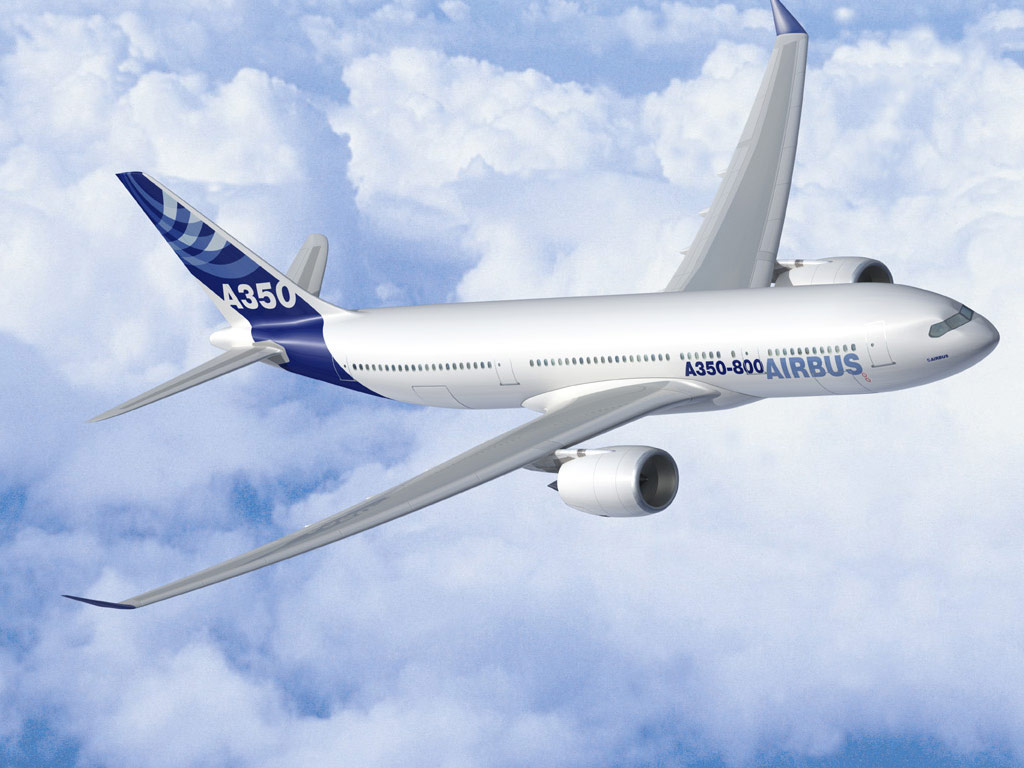
\includegraphics[height=50mm]{Figures/Airbus_A350.jpg}

% Title, author and degree
\vspace{1.0cm}
{\FontLb Thesis Title} \\ % <<<<< EDIT TITLE
%\vspace{0.2cm}
%{\FontMn Subtitle (optional)} \\
%\vspace{1.9cm}
\vspace{2.6cm}
{\FontMb Candidate Full Name} \\ % <<<<< EDIT NAME
\vspace{2.0cm}
{\FontSn \coverThesis} \\
\vspace{0.3cm}
{\FontLb Aerospace Engineering} \\ % <<<<< EDIT COURSE
\vspace{1.0cm}
{\FontSn %
\begin{tabular}{ll}
 \coverSupervisors: & Prof. Full Name 1 \\ % <<<<< EDIT NAME
                    & Dr. Full Name 2    % <<<<< EDIT NAME
\end{tabular} } \\
\vspace{1.0cm}
{\FontMb \coverExaminationCommittee} \\
\vspace{0.3cm}
{\FontSn %
\begin{tabular}{c}
\coverChairperson:     Prof. Full Name          \\ % <<<<< EDIT NAME
\coverSupervisor:      Prof. Full Name 1 (or 2) \\ % <<<<< EDIT NAME
\coverMemberCommittee: Prof. Full Name 3           % <<<<< EDIT NAME
\end{tabular} } \\
\vspace{1.5cm}
{\FontMb Month Year} \\ % <<<<< EDIT DATE (corresponds to date of oral examination)
%
\end{center}

 % file "Thesis_FrontCover.tex"
\cleardoublepage

% ----------------------------------------------------------------------
% Dedication page (optional)
% ----------------------------------------------------------------------
%%%%%%%%%%%%%%%%%%%%%%%%%%%%%%%%%%%%%%%%%%%%%%%%%%%%%%%%%%%%%%%%%%%%%%%%
%                                                                      %
%     File: Thesis_Dedication.tex                                      %
%     Tex Master: Thesis.tex                                           %
%                                                                      %
%     Author: Andre C. Marta                                           %
%     Last modified :  2 Jul 2015                                      %
%                                                                      %
%%%%%%%%%%%%%%%%%%%%%%%%%%%%%%%%%%%%%%%%%%%%%%%%%%%%%%%%%%%%%%%%%%%%%%%%

\null\vskip5cm%
\begin{flushright}
     Dedicated to someone special...
\end{flushright}
\vfill\newpage

 % file "Thesis_Dedication.tex"
\cleardoublepage

% ----------------------------------------------------------------------
%  Acknowledgments (optional)
% ----------------------------------------------------------------------
%%%%%%%%%%%%%%%%%%%%%%%%%%%%%%%%%%%%%%%%%%%%%%%%%%%%%%%%%%%%%%%%%%%%%%%%
%                                                                      %
%     File: Thesis_Acknowledgments.tex                                 %
%     Tex Master: Thesis.tex                                           %
%                                                                      %
%     Author: Andre C. Marta                                           %
%     Last modified :  2 Jul 2015                                      %
%                                                                      %
%%%%%%%%%%%%%%%%%%%%%%%%%%%%%%%%%%%%%%%%%%%%%%%%%%%%%%%%%%%%%%%%%%%%%%%%

\section*{\acknowledgments}

% Add entry in the table of contents as section
\addcontentsline{toc}{section}{\acknowledgments}

A few words about the university, financial support, research advisor, dissertation readers, faculty or other professors, lab mates, other friends and family...

 % file "Thesis_Acknowledgements.tex"
\cleardoublepage

% ----------------------------------------------------------------------
%  Abstract (both in English and Portuguese)
% ----------------------------------------------------------------------
%%%%%%%%%%%%%%%%%%%%%%%%%%%%%%%%%%%%%%%%%%%%%%%%%%%%%%%%%%%%%%%%%%%%%%%%
%                                                                      %
%     File: Thesis_Resumo.tex                                          %
%     Tex Master: Thesis.tex                                           %
%                                                                      %
%     Author: Andre C. Marta                                           %
%     Last modified :  2 Jul 2015                                      %
%                                                                      %
%%%%%%%%%%%%%%%%%%%%%%%%%%%%%%%%%%%%%%%%%%%%%%%%%%%%%%%%%%%%%%%%%%%%%%%%

\section*{Resumo}

% Add entry in the table of contents as section
\addcontentsline{toc}{section}{Resumo}

Inserir o resumo em Portugu\^{e}s aqui com o máximo de 250 palavras e acompanhado de 4 a 6 palavras-chave...

\vfill

\textbf{\Large Palavras-chave:} palavra-chave1, palavra-chave2,...

   % file "Thesis_Resumo.tex"
\cleardoublepage

%%%%%%%%%%%%%%%%%%%%%%%%%%%%%%%%%%%%%%%%%%%%%%%%%%%%%%%%%%%%%%%%%%%%%%%%
%                                                                      %
%     File: Thesis_Abstract.tex                                        %
%     Tex Master: Thesis.tex                                           %
%                                                                      %
%     Author: Andre C. Marta                                           %
%     Last modified :  2 Jul 2015                                      %
%                                                                      %
%%%%%%%%%%%%%%%%%%%%%%%%%%%%%%%%%%%%%%%%%%%%%%%%%%%%%%%%%%%%%%%%%%%%%%%%

\section*{Abstract}

% Add entry in the table of contents as section
\addcontentsline{toc}{section}{Abstract}

In Cloud environment, programming distributed solutions, covering interoperability between heterogeneous systems,
they are essentially based on SOA or REST technology, based on HTTP, XML and JSON. The problem is that these technologies
were developed in the web context where the main objective is the integration of existing systems and not programming
distributed with efficiency and performance as top concerns. How to compromise these two views in the global environment,
on cloud computing?\\

SOA and Web services are heavy and complex technologies. The popularity of REST is due more to its simplicity than to its
mapping the paradigm of services. However, any of them is not very efficient, based on HTTP and languages
text-based data description (XML and JSON). The result is that the description of Web Services (WSDL) and languages
high-level programming are inefficient and complex. The binary version of XML is no more than a compression
data only for transmission effect (compressed and decompressed on the issue at the reception). A solution used in this
work uses binary data format natively, does not require schema and the runtime environment uses Web Sockets,
much more efficient than HTTP, while maintaining some compatibility.\\

New solution is developed for distributed programming in cloud computing environment to develop
distributed applications, using  asymmetric interoperability, based on compliance and conformance and comparing this solution with the more classical solutions based on SOA and REST. The aim of this work explains this solution and its environment execution. Comparison with the corresponding solutions with technologies based on SOA (Web Services)
and REST.

\vfill

\textbf{\Large Keywords:} SOA, WSDL, REST, XML, JSON, HTTP, Web Sockets
 % file "Thesis_Abstract.tex"
\cleardoublepage

% ----------------------------------------------------------------------
%  Table of contents, list of tables, list of figures and nomenclature
% ----------------------------------------------------------------------

% Table of contents
%
\tableofcontents
\cleardoublepage

% List of tables
%
% Add entry in the table of contents as section
\phantomsection
\addcontentsline{toc}{section}{\listtablename}
% Generate list
\listoftables
\cleardoublepage

% List of figures
%
% Add entry in the table of contents as section
\phantomsection
\addcontentsline{toc}{section}{\listfigurename}
% Generate list
\listoffigures
\cleardoublepage

% Nomenclature
%
% entries of nomenclature list
%%%%%%%%%%%%%%%%%%%%%%%%%%%%%%%%%%%%%%%%%%%%%%%%%%%%%%%%%%%%%%%%%%%%%%%%
%                                                                      %
%     File: Thesis_Nomenclature.tex                                    %
%     Tex Master: Thesis.tex                                           %
%                                                                      %
%     Author: Andre C. Marta                                           %
%     Last modified : 21 Jan 2011                                      %
%                                                                      %
%%%%%%%%%%%%%%%%%%%%%%%%%%%%%%%%%%%%%%%%%%%%%%%%%%%%%%%%%%%%%%%%%%%%%%%%
%
% The definitions can be placed anywhere in the document body
% and their order is sorted by <symbol> automatically when
% calling makeindex in the makefile
%
% The \glossary command has the following syntax:
%
% \glossary{entry}
%
% The \nomenclature command has the following syntax:
%
% \nomenclature[<prefix>]{<symbol>}{<description>}
%
% where <prefix> is used for fine tuning the sort order,
% <symbol> is the symbol to be described, and <description> is
% the actual description.

% ----------------------------------------------------------------------
% Roman symbols [r]
\nomenclature[ru]{$\bf u$}{Velocity vector.}
\nomenclature[ru]{$u,v,w$}{Velocity Cartesian components.}
\nomenclature[rp]{$p$}{Pressure.}
\nomenclature[rC]{$C_D$}{Coefficient of drag.}
\nomenclature[rC]{$C_L$}{Coefficient of lift.}
\nomenclature[rC]{$C_M$}{Coefficient of moment.}

% ----------------------------------------------------------------------
% Greek symbols [g]
\nomenclature[g]{$\rho$}{Density.}
\nomenclature[g]{$\alpha$}{Angle of attack.}
\nomenclature[g]{$\beta$}{Angle of side-slip.}
\nomenclature[g]{$\mu$}{Molecular viscosity coefficient.}
\nomenclature[g]{$\kappa$}{Thermal conductivity coefficient.}

% ----------------------------------------------------------------------
% Subscripts [s]
\nomenclature[s]{$x,y,z$}{Cartesian components.}
\nomenclature[s]{$i,j,k$}{Computational indexes.}
\nomenclature[s]{$\infty$}{Free-stream condition.}
\nomenclature[s]{ref}{Reference condition.}
\nomenclature[s]{$n$}{Normal component.}

% ----------------------------------------------------------------------
% Supercripts [t]
\nomenclature[t]{T}{Transpose.}
\nomenclature[t]{*}{Adjoint.}

 % file "Thesis_Nomenclature.tex"
%
% Add entry in the table of contents as section
\phantomsection
\addcontentsline{toc}{section}{\nomname}
% Insert glossary/nomenclature section produced by MakeIndex
\printnomenclature
\cleardoublepage

% entries of glossary list
%%%%%%%%%%%%%%%%%%%%%%%%%%%%%%%%%%%%%%%%%%%%%%%%%%%%%%%%%%%%%%%%%%%%%%%%
%                                                                      %
%     File: Thesis_Glossary.tex                                        %
%     Tex Master: Thesis.tex                                           %
%                                                                      %
%     Author: Andre C. Marta                                           %
%     Last modified : 30 Oct 2012                                      %
%                                                                      %
%%%%%%%%%%%%%%%%%%%%%%%%%%%%%%%%%%%%%%%%%%%%%%%%%%%%%%%%%%%%%%%%%%%%%%%%
%
% The definitions can be placed anywhere in the document body
% and their order is sorted by <symbol> automatically when
% calling makeindex in the makefile
%
% The \glossary command has the following syntax:
%
% \glossary{entry}
%
% The \nomenclature command has the following syntax:
%
% \nomenclature[<prefix>]{<symbol>}{<description>}
%
% where <prefix> is used for fine tuning the sort order,
% <symbol> is the symbol to be described, and <description> is
% the actual description.

% ----------------------------------------------------------------------

\glossary{name={\textbf{MDO}},description={Multi-Disciplinar Optimization is an engineering technique that uses optimization methods to solve design problems incorporating two or more disciplines.}}

\glossary{name={\textbf{CFD}},description={Computational Fluid Dynamics is a branch of fluid mechanics that uses numerical methods and algorithms to solve problems that involve fluid flows.}}

\glossary{name={\textbf{CSM}},description={Computational Structural Mechanics is a branch of structure mechanics that uses numerical methods and algorithms to perform the analysis of structures and its components.}}

 % file "Thesis_Glossary.tex"

% Add entry in the table of contents as section
\phantomsection
\addcontentsline{toc}{section}{\glossaryname}
% Insert glossary section produced by MakeIndex
\printglossary
\cleardoublepage

% Set arabic numbering (1,2,...) after preface
%
\setcounter{page}{1}
\pagenumbering{arabic}

% ----------------------------------------------------------------------
%  Chapters
% ----------------------------------------------------------------------

%%%%%%%%%%%%%%%%%%%%%%%%%%%%%%%%%%%%%%%%%%%%%%%%%%%%%%%%%%%%%%%%%%%%%%%%
%                                                                      %
%     File: Thesis_Introduction.tex                                    %
%     Tex Master: Thesis.tex                                           %
%                                                                      %
%     Author: Andre C. Marta                                           %
%     Last modified :  2 Jul 2015                                      %
%                                                                      %
%%%%%%%%%%%%%%%%%%%%%%%%%%%%%%%%%%%%%%%%%%%%%%%%%%%%%%%%%%%%%%%%%%%%%%%%

\chapter{Introduction}
\label{chapter:introduction}
\section{Overview}
\label{section:overview}
This chapter gives information about the subject of the thesis, the area of interest with that subject and also general information about current solutions related that topic.

\section{Context}
\label{section:context}

Distributed applications are required in most of central application sectors including e-commerce, e-banking, e-learning, e-health, telecommunication and transportation\citep{thesis:introduction1}. This results that the Internet plays an important role in business, administration and our everyday activities. In distributed applications that share information between each other does not need to be built with same technologies. The fundamental problem is the programming of distributed applications with all the basic interoperability problems involves distributed platforms and heterogeneous components.

On the other hand, Clouds create a new challenge for distribution. They bring new opportunities such as scalability, dynamic instantiation, location independence, application management and multi-tenancy (several users using the same application independently)\citep{thesis:introduction2}. However, they also create distributed platforms and that’s why they need to be able to support distributed applications as easily as possible. That's make importance of interoperability in cloud environment because different cloud providers can have different properties and they need to communicate between each other.

The subject of thesis research current solutions of distributed applications and their implementation in cloud environment and propose the design of the alternative solution that is both simpler and more effective than existing ones.

Taking your Android mobile phone as an example, nowadays a huge part of the people use smartphones that are connected Internet that check news, weathercast or more information like that. Let’s say you have an application in your phone that informs you with current weathercast of your city. That application is most probably written in Java since your phone is using Android system and gets current weathercast over Internet that gets information from weathercast provider, so basically that application asks queries to weathercast provider over Internet and gets response data first and then parse that data and display information to your phone screen. During this data exchange happens, both your mobile phone and weathercast provider must understand each other even they don’t use the same language because the provider could be working in a Cloud provider and written in C\# language. The data is used in C\# and Java is not the same so they will not understand each other naturally. This interoperability (how to interconnect different programs written in different languages, running in different platforms) issue can be solved with current integration technologies such as SOA or REST using XML or JSON over HTTP and both platforms can communicate between each other. Finally you can get last weathercast information from your Android phone or your IPhone using same weathercast provider even they use totally different technologies.

\section{The problem}
\label{section:problem}

Distributed applications need to interact among themselves. In this respect, they need to solve the interoperability problems as any two systems that need to understand each other to achieve meaningful and useful collaboration. The traditional integration technologies, based on either SOA or REST as seen in Figure \ref{fig:soaprest}, is that they use the document concept as the foundation, with a data description language as the representation format and schema sharing as the interoperability mechanism (both sides use the same schema such XML Schema) or using previously known data types. Other factors, such as connectionless protocol (HTTP) and XML, JSON (and by extension SOA and REST) that do not support binary in its main features, because the solutions were also based on text (XML or JSON) and contextual information, are limited for many applications.

\begin{figure}[!htb]
  \centering
  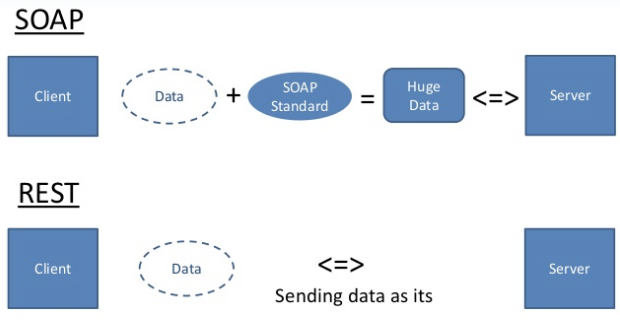
\includegraphics[width=0.9\textwidth]{Figures/soap-rest.png}
  \caption[SOAP and REST Approach.]{SOAP and REST Approach.}
  \label{fig:soaprest}
\end{figure}

The main problem of the traditional integration technologies creates coupling between the provider and the consumer, because both customer and provider are forced to implement full interoperability (for example, sharing a XML schema). This leads to a greater coupling than needed.

While solving data interoperability, the problem of using XML or JSON is that XML or JSON is inefficient in computer terms due to parsing data to build a DOM tree and validating schemas to validate structure of message.

The problem can be explained with an example, as described in the previous example in section \ref{section:context} that you can have two different technologies and they can communicate each other. In case if they use SOA architecture style (namely, SOAP Web Services) you need to use XML (Extensible Markup Language), which both languages can understand easily since, it is a common language. But still you have some steps to deal such as a stub, which is used by a client application to access a remote service. The stub looks like the service interface\citep{thesis:introduction3}; it generates an appropriate XML message and sends it over HTTP then you have XML message that can be read by your mobile phone or weathercast provider and parsed to build a DOM tree to be used. That can be done with sharing same schema to know structure of message. There are some problems with sharing schema which brings coupling problem between systems. So when you want to see weathercast on your phone, firstly your phone creates query message in XML using stub generator then uses HTTP for message transportation. The created message should be validated by schema because if it doesn't obey the schema rules, the provider can not understand the message. When message arrives to provider it validates message regarding the same schema and parses that XML message to own objects to understand it then provide response regarding the query, which is done by your phone application. There are some problems with using XML schema because your phone application or weathercast provider can not alter this schema without informing each other. That creates coupling between mobile application and weathercast provider. After message creation by weathercast provider, this response again needs to be converted to XML message using stub generator and send that response message to your phone. Now, your phone uses XML schema and XML parsers to understand XML message and uses these data to display information to you. As seen in that example it is not very easy to communicate systems that use totally different technologies. In case of REST, you can use different message format instead of XML, for example, JSON which is easier to parse and less heavier than XML, but in REST both languages need to know message structure, then they can parse and understand.

In case of REST, there are some differences. If your weathercast application uses REST to communicate with weathercast provider then you don’t need to create XML message to send weathercast provider. You can use other formats to send it using HTTP to server. Assume that you use JSON and your mobile phone creates query in JSON format then it needs to know unique URl of weather cast provider and HTTP verbs (GET, POST, PUT, and DELETE) because in REST, different HTTP methods can be used with using the same URl. When a message arrived to weathercast provider this message will be parsed with DOM parsers to understand query. In that case your phone and weathercast provider must know structure of JSON message than they can both understand each other. REST may seem more flexible, in the sense that, if the server changes the links it sends in the responses, the client will follow this change automatically by using the new links. However, the problem is that this is not as general as it may seem, since the client must be able to understand the structure of the responses. To achieve this, REST imposes the constraint that returns representations using standardized or pre-agreed media types. Your mobile phone application or weathercast provider can not alter this structure of JSON without informing each other. After a message parsed by provider then it creates response message in JSON format to send back your phone and now your phone displays weathercast to you.

Current integration technologies, based on either SOA or REST, is that they use a data description language as the representation format and schema sharing as the interoperability mechanism. Other factors, using a connectionless protocol (HTTP) and the lack of native support for binary data and contextual information limit for many applications, although they are not impeditive.

The main problems with using traditional integration technologies can be summerized as follows:
\begin{itemize}
  \item Data interoperability problems based on XML and JSON (Stub generation,DOM parsing)
  \item Service interoperabiliy problems based on SOA and REST(Coupling with schema sharing)
  \item The underlying protocol, usually HTTP, without binary support
\end{itemize}

These are the main problems with using traditional integration technologies. In section \ref{section:solution}, an alternative solution will be proposed to solve described problems.

\section{The solution}
\label{section:solution}

As a solution to the problems mentioned above like creating coupling between the provider and the consumer, because both customer and provider are forced to implement full interoperability (sharing schema), now think a new solution way with providing the maximum decoupling possible while ensuring the minimum interoperability requirements and allowing the client or the sender to changebility, as long as the actual used parts do not change. The current solutions that are described in section \ref{section:problem} use schema sharing to understand message structure with created unnecessary coupling, and what about using compliance (consumer must satisfy the requirements established by the provider to accept requests sent to it)\citep{compliance:def} and conformance (the provider must fulfill the expectations of the consumer regarding the effects of a request)\citep{comformance:def2} instead of sharing the same schema. Building interoperability on compliance and conformance avoids the problem of having to define schemas as separate documents and to agree upon them beforehand. As long as compliance and conformance hold, any two resources can interoperate, even if they were designed unbeknownst to each other. Another solution for performance instead of using XML or JSON, based on text which is heavy and hard to parse, uses binary directly for message transportation which reduce complexity improve performance. Again for performance, regarding message transportation, uses Web Sockets and HTTP/2 protocol (a binary protocol with small message frames) instead of using classical HTTP. Following chapters give more details and examples about the topics that are mentioned in current section.

\section{Contributions}
\label{section:contributions}
The goal of this dissertation is more than just an implementation and the value of this dissertation lie in the demonstration of conclusions, with respect to Web Services and REST.

The contributions are made in dissertation as follows:

\begin{itemize}
  \item Trying a new method for interoperability problem with using compliance and comformance which is not known and used very well in the market.
  \item The solution aimed to combining best features of SOA and REST.
  \item The solution will be demonstrated through experiments. Showing results that it is a better solution for application interoperability and also it is easier to implement. Also assessing performance to show advantage of using binary, with comparison current solutions.
\end{itemize}

\section{Organization}
\label{section:organization}

The organization of dissertation is prepared as follows:

\begin{itemize}
\item State of Art - Chapter 2 details some aspects of existing solutions for distributed systems for cloud environment, namely SOA, REST, text based data (XML and JSON). It also details about new tools that will be used, namely HTTP/2 and Web Sockets.
\item Interoperability - Chapter 3 starts describing interoperability and explaining different perspective from classical solutions to our new solution to overcome interoperability problem.
\item Architecture of the solution - Chapter 4 provides some insight on how our system can be used and gives a general overview of how and why it works.
\item Implementation - Chapter 5 goes more in depth on the inner workings of our system than the previous chapter and presents one implementation for our system.
\item Comparison with existing technologies - Chapter 6 presents the benchmarks used to evaluate our system with current solutions and the results obtained.
\item Conclusions - Chapter 7 summarizes the work described in this dissertation, the results achieved, and what are its main contributions. It also presents some possible future improvements to our proposed solution.
\end{itemize}
 % file "Thesis_Introduction.tex"
\cleardoublepage

%%%%%%%%%%%%%%%%%%%%%%%%%%%%%%%%%%%%%%%%%%%%%%%%%%%%%%%%%%%%%%%%%%%%%%%%
%                                                                      %
%     File: Thesis_State_of_the_art.tex                                %
%     Tex Master: Thesis.tex                                           %
%                                                                      %
%                                                                      %
%%%%%%%%%%%%%%%%%%%%%%%%%%%%%%%%%%%%%%%%%%%%%%%%%%%%%%%%%%%%%%%%%%%%%%%%

\chapter{State-of-the-art}
\label{chapter:stateofart}


%%%%%%%%%%%%%%%%%%%%%%%%%%%%%%%%%%%%%%%%%%%%%%%%%%%%%%%%%%%%%%%%%%%%%%%%
\section{Overview}
\label{section:overview}

(description of existing technologies and tools that you will use)
Existing Technologies

- SOA (Youtube)

- REST (YouTube)

Tools
Tomcat
.Net Framework 4.5

Language (C# - Java)
Deployment -
Azure Web Services Cloud Technoloies
Insert your chapter material here...

%%%%%%%%%%%%%%%%%%%%%%%%%%%%%%%%%%%%%%%%%%%%%%%%%%%%%%%%%%%%%%%%%%%%%%%%

\section{Web Services}
\label{section:webservices}

Web Services are exposed to the Internet for programmatic access. They are online APIs that you can call from your code.\\
When you want to call any API that written by someone else to your java code, you basically add jar or classes to
your class path and executions are done inside of machine or single environment. In the case of web services however
you have different pieces of code deployed over different machines and they call methods of each other over the network.
For example, you must have seen that different apps or games, which can post to your Facebook wall even these games,
not designed by Facebook. So you ask that how they can do that or how they can post to a wall of completely different
system or application. Basically they do this by calling online APIs. Companies like Facebook or Twitter publish web
services that let other developers call them from their code, so other application developers can actually write
code to consume these services and they can post things on Facebook or Twitter. They can read or access data from
Facebook or Twitter using the APIs of the web services that Facebook or Twitter has provided.\\
Web services are similar to web pages. For example Twitter has web side URL as “www.twitter.com“ when you access
this URL on your browser you get an HTML response that let you read and write tweets. They have HTML elements for
data and also CSS files for styling, this is because web pages that you see is made human conception.
They know that there is actually human is behind of browser on a laptop or devices who was reading these tweets
so they want to make sure about its format properly, so it is easy to access and read.
Twitter has also other URL as “api.twitter.com“ that does a lot of same things as “www.twitter.com“ does,
but it behaves a bit differently for instance this API gives you response which doesn’t have HTML or CSS code.
It contains data but it is xml or json format and there are specific URLs for different operations this is what
the developers can use from their code to read or write to twitter, so this data is actually very easy for
parsing and converting then using in their objects and their code for developers. In this case there is no need HTML
and CSS files.\\
There are primarily two different types of web services. One of these types called as SOA web service and another type
called as REST web service. SOA is older of these two and REST is newer entry to web services world, but both of them
are used popular. Next chapter will be focusing on SOA and REST web services.

%%%%%%%%%%%%%%%%%%%%%%%%%%%%%%%%%%%%%%%%%%%%%%%%%%%%%%%%%%%%%%%%%%%%%%%%
\section{SOA Web Services}
\label{section:soa}
DEFINITON

xXXX
https://books.google.fr/books/about/Understanding_Web_Services.html?id=SHSBri-rMyQC&redir_esc=y

EXAMPLE

Let’s start an example with java application. Let’s say we have implementation class and I want to share this implementation
class with other developer projects. How I would share this with a consumer class. The best way to share this implementation
class would be to contract it with an interface and other consumers would consume this class through this interface.
They would call implementation through interface so they get contract and they get the methods, arguments, written types
through interface. They actually call the methods of implementation class, so how this works in case of web service, let’s
say I have web service implementation and I want to share details of this web service to consumers. Is it works with an
interface? Probably it will not work because as we discussed before you don’t know what technology is consuming it. It might
be C# application or C++ application, so if you have a java web service you might want to give some kind of information that
its consumer respects to that technology and that can actually consume. Let’s say consumer is .Net and if I give this .Net
application a java interface then most probably it will not work because they are different technologies, so the technology
that I am going to share with web service consumer has to be technology independent. It should be something that any
application or any technology can understand so creators of SOA web service talked about that problem and what to give format
understandable by all technology with all consumers and decided with XML. So what you do is in case of web service, you
actually share that contract as an XML document. This XML document is actually called as WSDL.\\

[GRAPH]  -> interface similar to video\\

WSDL document contains the contract to web service and so that’s are the things you have to do when you create the web
service and you share WSDL document of that web service to the consumers, so this is not something you would have to do
it manually. You would do it manually but there are tools which generate WSDL for the web service but it is something that
you need to share this WSDL to consumers and it is a XML document, so it respective whatever application because applications
such as .Net, C++ or Java can all parse this XML and get to know about service information and typically the content of
this WSDL is kind of similar to an interface content. It has operations, arguments and types  to return that consumer
applications will have idea what to call and how to call.\\

[GRAPH] WSDL similar to video\\

The new question is that how this exchange happens, how you actually send this information, let’s say you have a method in
your java application and input argument is a string so you have a java string with you and you need to send to web service
and let’s say output return type is a list, so how you get this information because that could be .Net application and string
in java obviously different from string in C#. How do you exchange this between client app and web service?  When you exchange
information input argument or return type you need to exchange it in the format that all different technologies can understand
what you are passing and it should be able to send return type back in language that all these technologies can understand.
Again this format is XML. When you are sending any information across the network from a client to the web services and
return type back to the client, the data has to be in XML format. You are not really sending java string or a list. So it
has to be language natural format which is XML. There is specification about how you need to send all these different input
type and output argument basically any type needs to be send specific XML format.\\

It is a protocol that is a way in which both sender and receiver and this XML is called SOAP (Simple Object Access Protocol).
It is a way in which these different technologies can access objects can access data it supposedly simple so that a part
of the name is called simple object access protocol. So with this protocol all different technologies written in different
languages can kind of understand what they all taking about.\\

[GRAPH] SOAP\\

Now you know what is the mechanism you know what need to be send and you know how to send which is using SOAP protocol
but who does conversion? So for example you have your string object or complex object, so how do you convert it from java
object to a soap message? The conversion is actually done with intermedia class so this class takes care of converting all
your objects into a SOAP message. The whole method calls itself is actually done by SEI. The SEI access interface to your
web service endpoint so you have an interface at your client app to the service endpoint which translate all web service
call to a SOAP message and then it makes sure that the other things is able to understand this message. So we don’t have to
write this class and all the conversion ourselves. We can have it automatically generated for us. When you are making a web
service call you don’t worry about where the web service is. When you need to call, all you need to do is have this endpoint
interface and good thing about this service endpoint that you can actually have an interface that specific to what you are
developing. When you have a java application you will have a specific SEI for java application and it knows to convert java
objects to SOAP message. Let’s say your .Net application calling the same web service so you will have SEI for .NET that know
to convert .Net objects to SOAP message.\\

GRAPH SEI\\


%%%%%%%%%%%%%%%%%%%%%%%%%%%%%%%%%%%%%%%%%%%%%%%%%%%%%%%%%%%%%%%%%%%%%%%%
\section{Theoretical Model 1}
\label{section:theory1}

The research should be supported with a comprehensive list of references.
These should appear whenever necessary, in the limit, from the first to the last chapter.

A reference can be cited in any of the following ways:
%
\begin{itemize}
  \item Citation mode \#1 - \quad \cite{jameson:adjointns}
  \item Citation mode \#2 - \quad \citet{jameson:adjointns}
  \item Citation mode \#3 - \quad \citep{jameson:adjointns}
  \item Citation mode \#4 - \quad \citet*{jameson:adjointns}
  \item Citation mode \#5 - \quad \citep*{jameson:adjointns}
  \item Citation mode \#6 - \quad \citealt{jameson:adjointns}
  \item Citation mode \#7 - \quad \citealp{jameson:adjointns}
  \item Citation mode \#8 - \quad \citeauthor{jameson:adjointns}
  \item Citation mode \#9 - \quad \citeyear{jameson:adjointns}
  \item Citation mode \#10 - \quad \citeyearpar{jameson:adjointns}
\end{itemize}
%
Several citations can be made simultaneously as \citep{nocedal:opt,marta:ijcfd}. \\

This is often the default bibliography style adopted (numbers following the citation order), according to the options:\\
{\tt \textbackslash usepackage\{natbib\}} in file {\tt Thesis\_Preamble.tex},\\
{\tt \textbackslash bibliographystyle\{abbrvnat\}} in file {\tt Thesis.tex}.\\
%
Notice however that this style can be changed from numerical citation order to authors' last name with the options: \\
{\tt \textbackslash usepackage[numbers]\{natbib\}} in file {\tt Thesis\_Preamble.tex},\\
{\tt \textbackslash bibliographystyle\{abbrvunsrtnat\}} in file {\tt Thesis.tex}.


%%%%%%%%%%%%%%%%%%%%%%%%%%%%%%%%%%%%%%%%%%%%%%%%%%%%%%%%%%%%%%%%%%%%%%%%
\section{Theoretical Model 2}
\label{section:theory2}

Other models...
 % file "Thesis_State_of_the_art.tex"
\cleardoublepage

%%%%%%%%%%%%%%%%%%%%%%%%%%%%%%%%%%%%%%%%%%%%%%%%%%%%%%%%%%%%%%%%%%%%%%%%
%                                                                      %
%     File: Thesis_Implementation.tex                                  %
%     Tex Master: Thesis.tex                                           %

%%%%%%%%%%%%%%%%%%%%%%%%%%%%%%%%%%%%%%%%%%%%%%%%%%%%%%%%%%%%%%%%%%%%%%%%

\chapter{Implementation}
\label{chapter:implementation}

\section{Overview}
\label{section:overview}

This chapter describes the implementation details of the Binary Level Serialization, Receiver and Compliance, Message Transportation and Deployment. This chapter also gives experimental examples about new implementation to show that solution works in practice and that is better than XML or JSON regarding data binding and decoupling.

%%%%%%%%%%%%%%%%%%%%%%%%%%%%%%%%%%%%%%%%%%%%%%%%%%%%%%%%%%%%%%%%%%%%%%%%
\section{Binary Level Serialization}
\label{section:binaryLevelSerialization}

In this section, the implementation of the Binary level serialization will be presented. As in previous chapters, explained advantages of binary comparing to text-based solutions, it will be showed with some experimentation.

Computer languages have their own object types and special serialization algorithms for their object types, so when you are working with same language you can easily serialize an object and deserialize it back easily with other application which is written by same language.

When starting to work with different computer languages and their object types, most probably you have problem with serialization. You cannot use standard Java or .Net(C\#) object serialization, because different program languages use different algorithms  for serialization, that's why you’ll run into the problem with serialization. Let's explain that with a simple example. For example simple Person object such as in Listing ~\ref{lst:javaperson} has a binary representation which is not the same in .Net(Table \ref{tab:netserilazitaon}) and Java(Table \ref{tab:javaserilazitaon}).\\

\begin{lstlisting}[caption=Person Object, label=lst:javaperson]
  public class Person
  {
       public String name;
       public int age;
  }
\end{lstlisting}
Because both Java and .Net has different algorithms to serialize and deserialize their object classes and they are unaware of each other. The unique solution for that problem is avoid using standard serialization libraries for Java and .Net.
\begin{table}[]
\centering
\begin{tabular}{lllllllllllllll}
0   & 1   & 0   & 0   & 0   & 255 & 255 & 255 & 255 & 1   & 0   & 0   & 0   & 0   & 0  \\
0   & 0   & 12  & 2   & 0   & 0   & 0   & 73  & 83  & 101 & 114 & 105 & 97  & 108 & 105\\
122 & 97  & 116 & 105 & 111 & 110 & 32  & 116 & 101 & 115 & 116 & 44  & 32  & 86  & 101\\
114 & 115 & 105 & 111 & 110 & 61  & 49  & 46  & 48  & 46  & 48  & 46  & 48  & 44  & 32 \\
67  & 117 & 108 & 116 & 117 & 114 & 101 & 61  & 110 & 101 & 117 & 116 & 114 & 97  & 108\\
44  & 32  & 80  & 117 & 98  & 108 & 105 & 99  & 75  & 101 & 121 & 84  & 111 & 107 & 101\\
110 & 61  & 110 & 117 & 108 & 108 & 5   & 1   & 0   & 0   & 0   & 25  & 83  & 101 & 114\\
105 & 97  & 108 & 105 & 122 & 97  & 116 & 105 & 111 & 110 & 95  & 116 & 101 & 115 & 116\\
46  & 80  & 101 & 114 & 115 & 111 & 110 & 2   & 0   & 0   & 0   & 21  & 60  & 110 & 97 \\
109 & 101 & 62  & 107 & 95  & 95  & 66  & 97  & 99  & 107 & 105 & 110 & 103 & 70  & 105\\
101 & 108 & 100 & 20  & 60  & 97  & 103 & 101 & 62  & 107 & 95  & 95  & 66  & 97  & 99 \\
107 & 105 & 110 & 103 & 70  & 105 & 101 & 108 & 100 & 1   & 0   & 8   & 2   & 0   & 0  \\
0   & 6   & 3   & 0   & 0   & 0   & 4   & 74  & 111 & 104 & 110 & 32  & 0   & 0   & 0  \\
11  &     &     &     &     &     &     &     &     &     &     &     &     &     &    \\
\end{tabular}
\caption[.Net Serialization Person Object]{.Net Serialization Person Object}
\label{tab:netserilazitaon}
\end{table}

\begin{table}[]
\centering
\begin{tabular}{lllllllllllllll}
  -84 & -19 & 0   & 5  & 115 & 114 & 0   & 23   & 106 & 97  & 118 & 97  & 97  & 112  & 112 \\
  108 & 105 & 99  & 97 & 116 & 105 & 111 & 110  & 55  & 46  & 80  & 101 & 114 & 115  & 111 \\
  110 & 79  & -70 & 94 & 85  & -31 & -32 & -110 & 90  & 2   & 0   & 2   & 73  & 0    & 3 \\
  97  & 103 & 101 & 76 & 0   & 4   & 110 & 97   & 109 & 101 & 116 & 0   & 18  & 76   & 106 \\
  97  & 118 & 97  & 47 & 108 & 97  & 110 & 103  & 47  & 83  & 116 & 114 & 105 & 110  & 103 \\
  59  & 120 & 112 & 0  & 0   & 0   & 32  & 116  & 0   & 4   & 74  & 111 & 104 & 110  &     \\
\end{tabular}
\caption[Java Serialization Person Object]{Java Serialization Person Object}
\label{tab:javaserilazitaon}
\end{table}

After that experiment, creating a common algorithm for different languages is decided to be use instead of using standard serializer for Java or .Net that both languages could understand and easily serialize or deserialize.

The binary format is always the result of serializing data in each language. Each data has a tag, which describe data type and the number of bytes that follow and the serialized content. Recovering the serialized data is simply testing the tag to find the data type and then using the number of bytes and the serialized content.

A message to be sent is an object (in Java or .Net) that provides a serialization method, which basically builds a serialized message (an array of bytes) by successively  adding each of its components, serialized. This is done by invoking the methods of the serialization class for primitive data or by recursively invoking the serialization method of structured objects that constitute the message.

Instead of every class has their own serializer class, it is implemented with idea of centralizing the “object of primitive type to a sequence of bytes” and vice-versa methods in a single class is to avoid the need for every class to have these methods. Since they are static (they receive an object and return bytes, or vice versa), they can simply be concentrated in a static class (no instances) and invoked from anywhere.

The methods to serialize, receive a primitive object (integer, Boolean, etc) and an array of bytes, returning the array of bytes with the serialized object’s bytes appended. Therefore, each serialization method grows the byte array. When the user wants to send a message, that message is an instance of a class that has a method that knows how to serialize it, by invoking the serialization methods of the static class for each of its variables.
%We will show some examples of primitive type serialization.
%\begin{figure}[!htb]
%  \centering
%  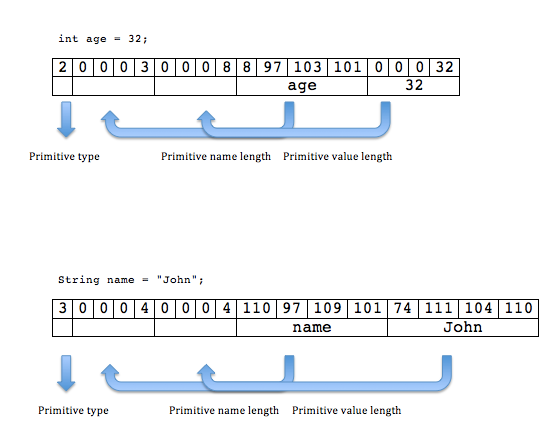
\includegraphics[width=0.9\textwidth]{Figures/binary.png}
%  \caption[Examples of primitive type serialization.]{Examples of primitive type serialization.}
%  \label{fig:examplebinary}
%\end{figure}

To examine the performance in serializing structured  data in binary and text-based data(XML,JSON), an experiment was designed using following hardware and software:
\begin{itemize}
\item 	Hardware: IMac(by Apple Inc.) with Intel Core i7 1,7 GHz and 8GB memory.
\item 	Operation System: Mac OS X version 10.11.4.
\item 	Java: version 1.8.
\end{itemize}
Current version of object serialization libraries were selected shown in the following:
\begin{itemize}
\item JAXB Serializer for XML serialization.
\item Jackson Serializer for JSON serialization.
\item OpenEXI for XML compression
\end{itemize}
The experiment was designed as follows:
\begin{itemize}
\item Ten kinds of query were prepared for weathercast provider. They were queries with ten different size of weather: 0, 100, 200, 300, 400, 500, 600, 700, 800, 900 weathercast query.
\item The serialized file was measured and the execution time was measured using System.currentTimeMillis() shown in Listing ~\ref{lst:timeserialize}.
\end{itemize}

\begin{lstlisting}[caption=Serialization program for testing, label=lst:timeserialize]
          long start = System.currentTimeMillis();
          Query q = new Query();
          for (int i = 0; i < 900; i++) {
              q.weathers.add(new Weather());
          }
          json = serialize(query);
          long end = System.currentTimeMillis();
          double time  =  (double) (end-start);
\end{lstlisting}

The avarage size of ten kinds of serialized files given in Table ~\ref{tab:binaryyy}.
\begin{table}
\centering
\begin{tabular}{ p{5.50cm} p{5.50cm} }
\toprule
\multicolumn{1}{l}{\textbf{Format}} & \textbf{Avarage (bytes)}\\
\midrule
\textbf{XML}    & 62008\\
\rowcolor{Gray}
\textbf{EXI}    & 3030\\
\textbf{JSON}   & 32036\\
\rowcolor{Gray}
\textbf{Binary} & 35984\\

\bottomrule
\end{tabular}
\caption[Sizes (in bytes) of several resource representations.]{Sizes (in bytes) of several resource representations.}
\label{tab:binaryyy}
\end{table}
\begin{figure}
    \begin{tikzpicture}
    \begin{axis}[
    title={Execution times for serialization of XML,JSON and Binary},
    xlabel={Number of weathercast query},
    ylabel={Execution time(ms.)},
    xmin=0, xmax=900,
    ymin=0, ymax=400,
    xtick={0,100,200,300,400,500,600,700,800,900},
    ytick={0,50,100,150,200,250,300,350,400},
    legend pos=north west,
    ymajorgrids=true,
    grid style=dashed,
]
\addplot[
    color=blue,
    mark=square,
    ]
    coordinates {
    (0,0)(100,33)(200,43.4)(300,63.2)(400,71.6)(500,90)(600,95.8)(700,99.2)(800,109)(900,111)
    };
   \addlegendentry{Binary}
\addplot[
    color=red,
    mark=square,
    ]
    coordinates {
   (0,0)(100,309)(200,324)(300,305)(400,330)(500,343)(600,303)(700,318)(800,328)(900,334)
    };
    \addlegendentry{JSON}
 \addplot[
    color=green,
    mark=square,
    ]
    coordinates {
   (0,0)(100,94.8)(200,100.2)(300,105.8)(400,107.4)(500,99.8)(600,103.6)(700,110.8)(800,109.4)(900,115.8)
    };
    \addlegendentry{XML}
\end{axis}
\end{tikzpicture}
\caption{Avarage Execution times for serialization of XML,JSON and Binary}
\label{fig:executiontime}
\end{figure}

From the point of the average size, the largest serialized file is obtained using XML, but EXI (Efficient XML Interchange) that use compression technology has best serialized file size when compared with others. But it does not reduce the parsing time, since text need to be recovered. On the other hand, Binary and JSON have very similar serialized file size. From the point of execution time binary serialization spends less time when compared with the others as seen in Figure~\ref{fig:executiontime}. From quantative aspects, the size of binary-based serialized data is better than XML-based and JSON-based serialization since there is no schema required and also in term of data binding, the binary-based serialization gives us big advantage with removing stub generation and DOM inspection.
%%%%%%%%%%%%%%%%%%%%%%%%%%%%%%%%%%%%%%%%%%%%%%%%%%%%%%%%%%%%%%%%%%%%%%%%

\section{Receiver and Compliance}
\label{section:compliance}

Compliance is done at the binary level, with primitive components. It is done both formal argument of the receiver method and received message. Only the components that match are assigned to the formal argument of the operation. Two partners will be able to communicate as long as the sender complies with receiver and the receiver conforms to what the sender expects and it supports all the features that the sender requires.

When a suitable operation is found, the server will complete operation and create a response for client. The system also supports optional components, which use the formal argument component if optional fields don't have value or different value. Therefore, the serialization methods in the static serialization class should include the name of the component, whether it is mandatory (with annotation), the type (encoded in the tag) and the value. Each primitive data type can have mandatory annotation. Messages sent use only with mandatory values. Serialized formal arguments can use both mandatory and non-mandatory. The receiver has always a default value for the message, so for the data that don't have mandatory annotation it will always use default value.

Let's explain that with an experiment. For that experiments there will be demonstration of 2 consumers (one developed with C\# and another with Java) and 2 providers (one developed with C\# and another with Java). General properties of 2 the consumers can be seen in Table ~\ref{tab:consumerProp}, then the properties of the providers also can be seen in Table ~\ref{tab:providerProp}


\begin{table}
\centering
\begin{tabular}{ p{5.50cm} p{5.50cm} p{5.50cm}}
\toprule
\multicolumn{1}{l}{\textbf{Device}} & \textbf{Role} & \textbf{Development technology}\\
\midrule
Mobile 1  \textbf{(Windows Mobile)}  & Consumer & C\# \\
\rowcolor{Gray}
Mobile 2  \textbf{(Android  Mobile)} & Consumer & Java \\
\bottomrule
\end{tabular}
\caption[General properties of the consumers for experiment.]{General properties of the consumers for experiment}
\label{tab:consumerProp}
\end{table}

\begin{table}
\centering
\begin{tabular}{ p{2.00cm} p{7.00cm} p{7.00cm}}
\toprule
\multicolumn{1}{l}{ } & \textbf{Cloud Server 1} & \textbf{Cloud Server 2}\\
\midrule
 \textbf{Role}                  & Provider       & Provider       \\
 \rowcolor{Gray}
 \textbf{Development technology}& .Net(C\#)      & Java            \\
 \textbf{Server technology}     & IIS 7.0 Server & Tomcat 8 Server \\
 \rowcolor{Gray}
 \textbf{Url}                   & http://csharpserverthesis.azurewebsites.net/ & http://javatomcatthesis.azurewebsites.net/ \\
\bottomrule
\end{tabular}
\caption[General properties of the providers for experiment.]{General properties of the providers for experiment}
\label{tab:providerProp}
\end{table}

Windows Mobile application (in Listing \ref{lst:wmobile}) sends 2 different query messages ({\tt Query1} as seen in Listing \ref{lst:query1} and {\tt Query2} as seen in Listing \ref{lst:query2}) to Cloud1 and Cloud2 providers. Android Mobile application (in Listing \ref{lst:andmobile}) sends a query message({\tt Query3} as seen in Listing \ref{lst:query3}) to Cloud 1 and Cloud 2 providers. If the receiver conforms to what the sender expects then there is compliance, the message received is partially assigned to that argument and the operation invoked.

\begin{lstlisting}[caption=Windows Mobile application, label=lst:wmobile]
  class Program
      {
          static void Main(string[] args)
          {
              Query1 q = new Query1();
              Message msg = new Message(q);
              string msgToSend = msg.Seriliaze();
              JavaWebServiceClient service = new JavaWebServiceClient();
              // Show result from server
              Console.WriteLine(" Result From Server: \n" + service.GetResult(msgToSend));
              Console.ReadLine();
          }

      }
\end{lstlisting}

\begin{lstlisting}[caption=Android Mobile application, label=lst:andmobile]
  public static void main(String[] args) throws Exception {
       final ChatClientEndpoint clientEndPoint = new ChatClientEndpoint(new URI("ws://javatomcatthesis.azurewebsites.net/JavaWebServerWebSocket-1.0/javawsendpoint"));
       clientEndPoint.addMessageHandler(new ChatClientEndpoint.MessageHandler() {
                   public void handleMessage(String message) {
                       System.out.println(message);
                   }
               });
         Query3 q = new Query3();;
         Message msg = new Message(q);
         byte[] msgToSend =  msg.SeriliazeBinary();
           clientEndPoint.sendMessage(msgToSend);
           Thread.sleep(30000);

   }
\end{lstlisting}

\begin{lstlisting}[caption=.Net provider [AvaliableMethod] notation in Receiver Class, label=lst:cserver]
  namespace CSharpWebServer.ist.enesuysal.thesis
  {
    public class Receiver
    {
        [AvaliableMethod]
        public void AvaliableMethod(Weather1 weather1){
        }
        [AvaliableMethod]
        public void AvaliableMethod(Weather2 weather2){
        }
        [AvaliableMethod]
        public void AvaliableMethod(Weather3 weather3){
        }
    }
  }
\end{lstlisting}

\begin{lstlisting}[caption=Java provider @AvaliableMethod notation in Receiver Class, label=lst:jaserver]
  package ist.enesuysal.thesis;
  public class Receiver
  {
    @AvaliableMethod
    public void AvaliableMethod(Weather4 weather4) {
    }
    @AvaliableMethod
    public void AvaliableMethod(Weather5 weather5) {
    }
    @AvaliableMethod
    public void AvaliableMethod(Weather6 weather6) {
    }
  }
\end{lstlisting}

\begin{lstlisting}[caption=Details of Query1 Object, label=lst:query1]
    public class WeatherQuery1
    {
      public String country = "Portugal";
      public String city = "Lisbon";
    }
\end{lstlisting}
\begin{lstlisting}[caption=Details of Query2 Object, label=lst:query2]
  public class WeatherQuery2
  {
    public int cityCode = 35121;
  }
\end{lstlisting}

\begin{lstlisting}[caption=Details of Query3 Object, label=lst:query3]
  public class WeatherQuery3
  {
    public double latitude = 38.736946;
    public double longitude  = -9.142685;
  }
\end{lstlisting}

Providers have operations with an input parameter of each of its operations. Operations have at most one argument, which can be structured. Matching will be done with message from consumer and input parameter of operations.  Input parameters of operations in each server can be seen in Table \ref{tab:providerinput}

\begin{table}
\centering
\begin{tabular}{ p{5.50cm} p{5.50cm}}
\toprule
\multicolumn{1}{l}{\textbf{Cloud Server 1}} & \textbf{Cloud Server 2} \\
\midrule
Weather1 (in Listing \ref{lst:weather1}) & Weather4 (in Listing \ref{lst:weather4}) \\
\rowcolor{Gray}
Weather2 (in Listing \ref{lst:weather2}) & Weather5 (in Listing \ref{lst:weather5}) \\
Weather3 (in Listing \ref{lst:weather3}) & Weather6 (in Listing \ref{lst:weather6}) \\
\bottomrule
\end{tabular}
\caption[Information about input parameter of operations in the provider for experiment.]{Information about input parameter of operations in the provider for experiment.}
\label{tab:providerinput}
\end{table}

\begin{lstlisting}[caption=Details of Weather Object, label=lst:weather1]
  public class Weather1
    {
      [Mandatory]
      public String country = "Portugal";
      [Mandatory]
      public String city = "Braga";
    }
\end{lstlisting}
\begin{lstlisting}[caption=Details of Weather2 Object, label=lst:weather2]
  public class Weather2
    {
      [Mandatory]
      public int cityCode = 35121;
      public String country = "Portugal";
      public String city = "Lisbon";
    }
\end{lstlisting}
\begin{lstlisting}[caption=Details of Weather3 Object, label=lst:weather3]
  public class Weather3
    {
      [Mandatory]
      public String country = "Portugal";
      [Mandatory]
      public String city = "Braga";
      public int cityCode = 351253;
      public double latitude = 41.530918;
      public double longitude  = -8.780565;
    }
\end{lstlisting}
\begin{lstlisting}[caption=Details of Weather4 Object, label=lst:weather4]
  public class Weather4
  {
    @Mandatory
    public String country = "Portugal";
    @Mandatory
    public String city = "Lisbon";
    public double latitude = 38.736946;
    public double longitude  = -9.142685;
  }
\end{lstlisting}
\begin{lstlisting}[caption=Details of Weather5 Object, label=lst:weather5]
  public class Weather5
  {
    @Mandatory
    public double latitude = 38.736946;
    @Mandatory
    public double longitude  = -9.142685;
  }
\end{lstlisting}
\begin{lstlisting}[caption=Details of Weather6 Object, label=lst:weather6]
  public class Weather5
  {
    @Mandatory
    public int cityCode = 35121;
  }
\end{lstlisting}

Lets start with Windows mobile application (Mobile 1); to explain compliance and conformance concepts, by providing a message with {\tt Query1} (in Listing \ref{lst:query1}) and sending it to .Net cloud provider (Cloud Server 1).
{\tt Weather1} object in Cloud 1 provider will not be mapped to {\tt Query1}, because {\tt Weather1} in Cloud 1 provider has 2 mandatory fields as seen in Listing \ref{lst:weather1} {\tt country} and {\tt city} fields do not have same value. {\tt Weather2} in Cloud 1 provider has 3 fields one mandatory other two are optional as seen in Listing \ref{lst:weather2} , since mandatory field is not in the {\tt Query1}, mapping will not be occur. {\tt Weather3} object in Cloud 1 provider also will not be mapped to {\tt Query1}, because {\tt Weather3} in Cloud 1 has 2 mandatory fields and 3 optional fields as seen in Listing \ref{lst:weather3}, but mandatory {\tt city} field does not have the same value as in {\tt city} field in {\tt Query1}. No suitable operation is found, the server will not complete operation and create a response for consumer in Cloud Server 1. Next step, let's try sending {\tt Query1} to Cloud Server 2 to check if there is any compliable operation. {\tt Weather4} object in Cloud 2 provider will be mapped to {\tt Query1} and compliance hold, because {\tt Weather4} in Cloud 2 has 2 mandatory fields and 2 optional fields as seen in Listing \ref{lst:weather4} and {\tt city} and {\tt country} fields have same value with the {\tt Query1}. The optional fields in {\tt Weather4} does not exist in {\tt Query1}, but that is not important since they are optional and they will be used with their default values.  Now suitable operation is found, the server will complete operation and create a response for client in Cloud Server 2. Now, what about when sending {\tt Query2} (in Listing) with Windows mobile application to Cloud 1 and Cloud 2 providers. {\tt Weather1} object in Cloud 1 provider will not be mapped to {\tt Query2} because {\tt Weather1} has 2 mandatory fiels and these fields are not exist in {\tt Query2}. {\tt Weather2} object in Cloud 1 provider will be mapped to {\tt Query2} because, {\tt Weather2} in Cloud 1 provider has 1 mandatory fields and 2 optional fields and {\tt cityCode} field has same value with the {\tt Query2}. The optional fields in {\tt Weather2} does not exist in {\tt Query2}, but that is not important since they are optional and they will be used with their default values. {\tt Query2} message will be complied with {\tt Weather2}, the server will complete operation and create a response for client in Cloud Server 1.

As explained above, sending {\tt Query1} message in Windows phone application will be mapped in Java weather provider and return result message after compliance. {\tt Query2} message in Windows phone application will be mapped in .Net weather provider and return result message after compliance.

The consumer does not need to be written in C\#. it can be written in Java or other language. Lets show implementation of Android phone application (Mobile 2).  This application has {\tt Query3} as seen in Listing \ref{lst:query3} and it will send that query message to Cloud 1 and Cloud 2 providers. Because of similar reasons explained before, any operation in Cloud 1 provider will not be mapped to {\tt Query3} because mandatory fields of {\tt Weather1}, {\tt Weather2} or {\tt Weather3} are not exist in {\tt Query3}. Any operation in Cloud 2 provider also will not be mapped with {\tt Query3}, because again mandatory fields of {\tt Weather4}, {\tt Weather5} or {\tt Weather6} are not exist in Query3.

The results that are explained above about partial assignment of Mobile 1 and Mobile 2 applications can be seen in Table \ref{tab:resultss} and in Table \ref{tab:resultss2}.

\begin{table}
\centering
\begin{tabular}{ p{2.00cm} p{2.00cm} p{2.00cm} p{2.00cm} p{2.00cm} p{2.00cm} p{2.00cm}}
\toprule
\multicolumn{1}{l}{}&{\textbf{Weather1}} & \textbf{Weather2} & \textbf{Weather3} & \textbf{Weather4} & \textbf{Weather5} & \textbf{Weather6} \\
\midrule
Query 1 & - & - & - & + & - & -\\
\rowcolor{Gray}
Query 2 & - & + & - & + & - & +\\
Query 3 & - & - & - & - & - & -\\
\bottomrule
\end{tabular}
\caption[Compliance and Conformance between Query message and Weather objects .]{Compliance and Conformance between Query message and Weather objects.}
\label{tab:resultss}
\end{table}

\begin{table}
\centering
\begin{tabular}{ p{2.50cm} p{2.50cm} p{2.50cm} p{2.50cm}}
\toprule
\multicolumn{1}{l}{}&{} & \textbf{Cloud Server 1} & \textbf{Cloud Server 2} \\
\midrule
Mobile 1 & Query 1 & No  & Yes\\
         & Query 2 & Yes & Yes\\
\rowcolor{Gray}
Mobile 2 & Query 3 & No  & No\\
\bottomrule
\end{tabular}
\caption[Compliance and Conformance between Cloud Servers and Mobile phones.]{Compliance and Conformance between Cloud Servers and Mobile phones.}
\label{tab:resultss2}
\end{table}

The demonstration in this section, show that provided solution is an alternative solution to XML, JSON, WSDL and REST. The example that presented here, involves compliance or conformance, that it works and that it allows changes to the client and to the server without informing both sides.

 %To clarify the compliance, the idea is to serialize the argument (only one, but it can be structured) of each operation of a service(receiving object). This acts like a default value, against which the message received is matched. A service receiving a message matches it against the argument of each operation, until it finds one, assigns the message to that argument (partial assignment) and runs the operation, returning eventually a result.

%When checking for compliance, a component in the message with the same name as a component in the operation’s argument matches it and can be assigned to it (if the message complies with the argument, as a whole). If not, it is ignored. If a component in the argument is not matched by any of the message’s components and is optional , retains the argument’s value (which acts as a default value). If all non-optional  components in the argument are matched, there is compliance, the matching components of the message are assigned to those of the argument with the same name and those that do not match are ignored. Thus the designation partial assignment.

%%%%%%%%%%%%%%%%%%%%%%%%%%%%%%%%%%%%%%%%%%%%%%%%%%%%%%%%%%%%%%%%%%%%%%%%
\section{Message Transportation}
\label{section:messageTransfer}

Transferring the array of bytes from sender to receiver requires a binary channel like Web Sockets (HTTP2) or more classical way by encoding and decoding the binary array with BASE64 and then use typical HTTP-based solutions (Web Services or REST). The classical solution is non-optimal compared to the other ones, but it is easier to implement with existent tools.

Message Transportation in this solution is done with essentially JavaScript and Web Sockets, to circumvent some of the limitations of HTTP. But also the solution supports classical way by encoding and decoding the binary array with BASE64 and then using typical HTTP-based solutions.

Web Sockets are chosen technology for implementation because they are fundamental in the efficient support for binary data removes this restriction, increases performance. They use the protocol upgrade feature of HTTP and provide a substantial degree of compatibility with existing systems. Now they are part of the HTML5 world, servers and firewalls are increasingly supporting them and remove this restriction, adds binary support and increases performance.

\begin{figure}[!htb]
  \centering
  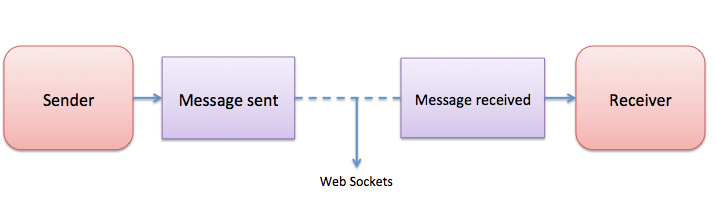
\includegraphics[width=0.5\textwidth]{Figures/websocket.png}
  \caption[Message Transportation.]{Message Transportation.}
  \label{fig:websocket}
\end{figure}

To examine the performance in HTTP-based solutions and Web Sockets, an experiment was designed using following hardware and software:

\begin{itemize}
\item 	Hardware: IMac(by Apple Inc.) with Intel Core i7 1,7 GHz and 8GB memory.
\item 	Operation System: Mac OS X version 10.11.4.
\item 	Java: version 1.8.
\end{itemize}

The experiment was designed as follows:
\begin{itemize}
\item Ten kinds of query were prepared for weathercast provider. They were queries with 6 different size of weather: 10, 100, 500, 1000, 5000, 10000 weathercast query.
\end{itemize}

\begin{figure}
\begin{tikzpicture}
\begin{axis}[
    ybar,
    enlargelimits=0.15,
    legend style={at={(0.5,-0.15)},
      anchor=north,legend columns=1},
    ylabel={Time},
    symbolic x coords={10,100,500,1000,5000,10000},
    xtick=data,
    nodes near coords,
    nodes near coords align={vertical},
    ]
\addplot coordinates {(10,17) (100,110) (500,520) (1000,1050) (5000,5180) (10000,10520) };
\addplot coordinates {(10,13) (100,19) (500,69) (1000,116) (5000,520) (10000,1019)};

\legend{HTTP-based(Web Service),Web Socket}
\end{axis}
\end{tikzpicture}
\caption{Avarage Times(in ms) of HTTP-based solutions and WebSocket.}
\label{fig:executiontimewebsocket}
\end{figure}

\begin{table}
\centering
\begin{tabular}{ p{5.50cm}p{5.50cm} p{5.50cm} }
\toprule
\multicolumn{1}{l}{\textbf{Nb of Message}} & \textbf{Web Service(HTTP) (in ms)} & \textbf{WebSocket(in ms)}\\
\midrule
\ 10    & 17    & 13\\
\ 100   & 110   & 19\\
\ 500   & 520   & 69\\
\ 1000  & 1050  & 116\\
\ 5000  & 5180  & 520\\
\ 10000 & 10520 & 1019\\

\bottomrule
\end{tabular}
\caption[Avarage Times(in ms) of HTTP-based solutions and WebSocket.]{Times (in ms) of HTTP-based solutions and WebSocket.}
\label{tab:websov}
\end{table}

As seen in Table \ref{tab:websov} and in Figure \ref{fig:executiontimewebsocket}, there is a big difference between the HTTP-based solutions and Web Sockets. It is clear to see using Web sockets technology adds a lot difference in performance aspect. Web Sockets also removes the limitations of HTTP which adds binary support and increases performance.

%%%%%%%%%%%%%%%%%%%%%%%%%%%%%%%%%%%%%%%%%%%%%%%%%%%%%%%%%%%%%%%%%%%%%%%%

\section{Deployment}
\label{section:deployment}

The solution is developed and in two different languages that are .NET and Java. The solution is deployed to Microsoft Azure Cloud. The reason choosing Microsoft Azure Cloud instead of other providers is because Microsoft provide free access to their App Servers of Azure with student subscription account. Another reason, .Net and Java technologies can be deployed using the same platform. Microsoft Azure support Java and .Net and that's way 2 different provider will be in the same platform. The Azure application servers support Web Sockets, which is also benefit to test new solution using Web Sockets in cloud environment. .Net client can send a message to Java provider over the cloud by using Web Sockets technology and also Java client can send message to .Net provider. Using Microsoft Azure Cloud technologies allowed us to test the project in cloud environment. The characteristics of Java application server and .Net application server can be seen in Figure~\ref{fig:javaserver} and in Figure~\ref{fig:netserver}

\begin{figure}[!htb]
  \centering
  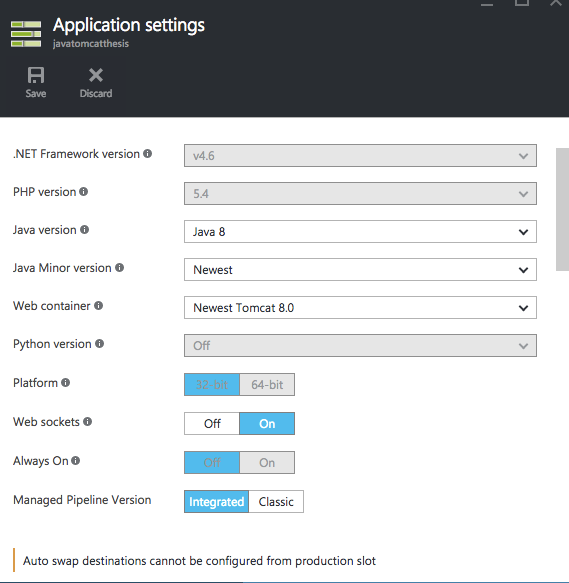
\includegraphics[width=0.7\textwidth]{Figures/javaserver.png}
  \caption[The characteristics of Java application server.]{The characteristics of Java application server.}
  \label{fig:javaserver}
\end{figure}

\begin{figure}[!htb]
  \centering
  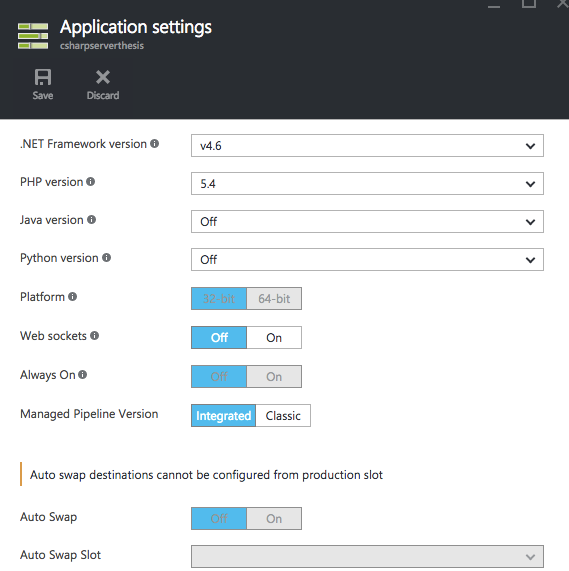
\includegraphics[width=0.7\textwidth]{Figures/dotnetserver.png}
  \caption[The characteristics of .Net application server.]{The characteristics of .Net application server.}
  \label{fig:netserver}
\end{figure}
 % file "Thesis_Implementation.tex"
\cleardoublepage

%\input{Thesis_new_file} % add new .tex files for new chapters
% \cleardoublepage

%\input{Thesis_new_file} % add new .tex files for new chapters
% \cleardoublepage

%\input{Thesis_new_file} % add new .tex files for new chapters
% \cleardoublepage

%%%%%%%%%%%%%%%%%%%%%%%%%%%%%%%%%%%%%%%%%%%%%%%%%%%%%%%%%%%%%%%%%%%%%%%%
%                                                                      %
%     File: Thesis_Results.tex                                         %
%     Tex Master: Thesis.tex                                           %
%                                                                      %
%     Author: Andre C. Marta                                           %
%     Last modified :  2 Jul 2015                                      %
%                                                                      %
%%%%%%%%%%%%%%%%%%%%%%%%%%%%%%%%%%%%%%%%%%%%%%%%%%%%%%%%%%%%%%%%%%%%%%%%

\chapter{Results}
\label{chapter:results}

Insert your chapter material here...


%%%%%%%%%%%%%%%%%%%%%%%%%%%%%%%%%%%%%%%%%%%%%%%%%%%%%%%%%%%%%%%%%%%%%%%%
\section{Problem Description}
\label{section:problem}

Description of the baseline problem...


%%%%%%%%%%%%%%%%%%%%%%%%%%%%%%%%%%%%%%%%%%%%%%%%%%%%%%%%%%%%%%%%%%%%%%%%
\section{Baseline Solution}
\label{section:baseline}

Analysis of the baseline solution...


%%%%%%%%%%%%%%%%%%%%%%%%%%%%%%%%%%%%%%%%%%%%%%%%%%%%%%%%%%%%%%%%%%%%%%%%
\section{Enhanced Solution}
\label{section:enhanced}

Quest for the optimal solution...


% ----------------------------------------------------------------------
\subsection{Figures}
\label{subsection:figures}

Insert your section material and possibly a few figures...

Make sure all figures presented are referenced in the text!


% ----------------------------------------------------------------------
\subsubsection{Images}
\label{subsection:images}

\begin{figure}[!htb]
  \centering
  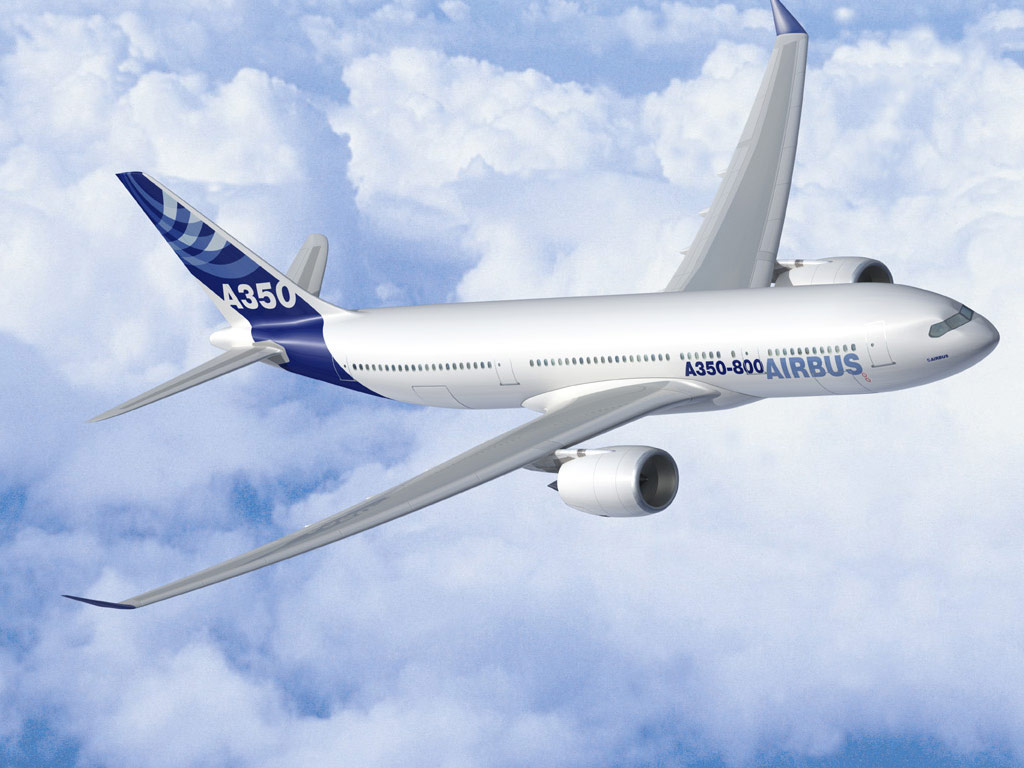
\includegraphics[width=0.25\textwidth]{Figures/Airbus_A350.jpg}
  \caption[Caption for figure in TOC.]{Caption for figure.}
  \label{fig:airbus1}
\end{figure}

\begin{figure}[!htb]
  \begin{subfigmatrix}{2}
    \subfigure[Airbus A320]{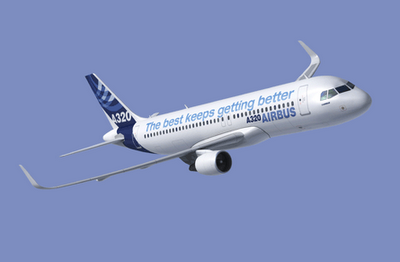
\includegraphics[width=0.49\linewidth]{Figures/Airbus_A320_sharklets.png}}
    \subfigure[Bombardier CRJ200]{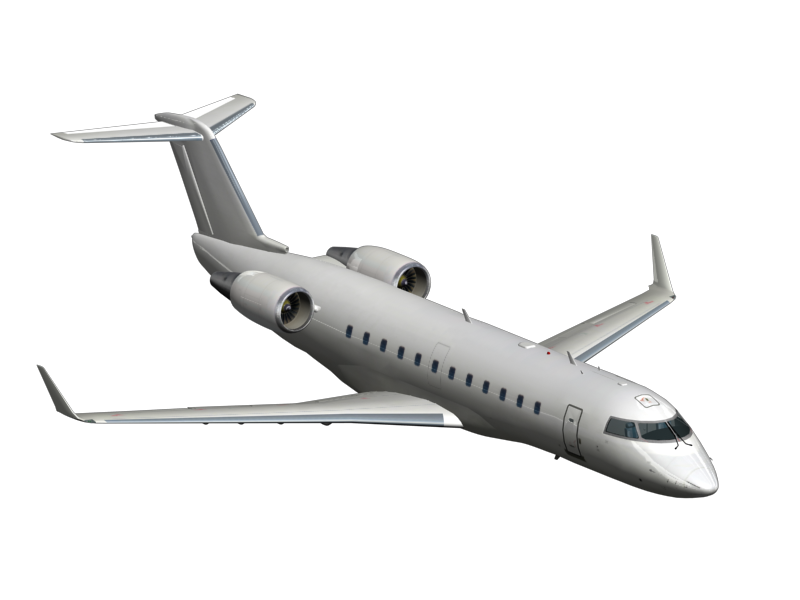
\includegraphics[width=0.49\linewidth]{Figures/Bombardier_CRJ200.png}}
  \end{subfigmatrix}
  \caption{Some aircrafts.}
  \label{fig:aircrafts}
\end{figure}

Make reference to Figures \ref{fig:airbus1} and \ref{fig:aircrafts}.

By default, the supported file types are {\it .png,.pdf,.jpg,.mps,.jpeg,.PNG,.PDF,.JPG,.JPEG}.

See \url{http://mactex-wiki.tug.org/wiki/index.php/Graphics_inclusion} for adding support to other extensions.


% ----------------------------------------------------------------------
\subsubsection{Drawings}
\label{subsection:drawings}

Insert your subsection material and for instance a few drawings...

The schematic illustrated in Fig.~\ref{fig:algorithm} can represent some sort of algorithm.

\begin{figure}[!htb]
  \centering
  \scriptsize
%  \footnotesize 
%  \small
  \setlength{\unitlength}{0.9cm}
  \begin{picture}(8.5,6)
    \linethickness{0.3mm}

    \put(3,6){\vector(0,-1){1}}
    \put(3.5,5.4){$\bf \alpha$}
    \put(3,4.5){\oval(6,1){}}
    %\put(0,4){\framebox(6,1){}}
    \put(0.3,4.4){Grid Generation: \quad ${\bf x} = {\bf x}\left({\bf \alpha}\right)$}

    \put(3,4){\vector(0,-1){1}}
    \put(3.5,3.4){$\bf x$}
    \put(3,2.5){\oval(6,1){}}
    %\put(0,2){\framebox(6,1){}}
    \put(0.3,2.4){Flow Solver: \quad ${\cal R}\left({\bf x},{\bf q}\left({\bf x}\right)\right) = 0$}

    \put(6.0,2.5){\vector(1,0){1}}
    \put(6.4,3){$Y_1$}

    \put(3,2){\vector(0,-1){1}}
    \put(3.5,1.4){$\bf q$}
    \put(3,0.5){\oval(6,1){}}
    %\put(0,0){\framebox(6,1){}}
    \put(0.3,0.4){Structural Solver: \quad ${\cal M}\left({\bf x},{\bf q}\left({\bf x}\right)\right) = 0$}

    \put(6.0,0.5){\vector(1,0){1}}
    \put(6.4,1){$Y_2$}

    %\put(7.8,2.5){\oval(1.6,5){}}
    \put(7.0,0){\framebox(1.6,5){}}
    \put(7.1,2.5){Optimizer}
    \put(7.8,5){\line(0,1){1}}
    \put(7.8,6){\line(-1,0){4.8}}
  \end{picture}
  \caption{Schematic of some algorithm.}
  \label{fig:algorithm}
\end{figure}


% ----------------------------------------------------------------------
\subsection{Equations}
\label{subsection:equations}

Equations can be inserted in different ways.

The simplest way is in a separate line like this

\begin{equation}
  \frac{{\rm d} q_{ijk}}{{\rm d} t} + {\cal R}_{ijk}({\bf q}) = 0 \,.
\label{eq:ode}
\end{equation}

If the equation is to be embedded in the text. One can do it like this ${\partial {\cal R}}/{\partial {\bf q}}=0$.

It may also be split in different lines like this

\begin{eqnarray}
  {\rm Minimize}   && Y({\bf \alpha},{\bf q}({\bf \alpha}))            \nonumber           \\
  {\rm w.r.t.}     && {\bf \alpha} \,,                                 \label{eq:minimize} \\
  {\rm subject~to} && {\cal R}({\bf \alpha},{\bf q}({\bf \alpha})) = 0 \nonumber           \\
                   &&       C ({\bf \alpha},{\bf q}({\bf \alpha})) = 0 \,. \nonumber
\end{eqnarray}

It is also possible to use subequations. Equations~\ref{eq:continuity}, \ref{eq:momentum} and \ref{eq:energy} form the Naver--Stokes equations~\ref{eq:NavierStokes}.

\begin{subequations}
    \begin{equation}
    \frac{\partial \rho}{\partial t} + \frac{\partial}{\partial x_j}\left( \rho u_j \right) = 0 \,,
    \label{eq:continuity}
    \end{equation}
    \begin{equation}
    \frac{\partial}{\partial t}\left( \rho u_i \right) + \frac{\partial}{\partial x_j} \left( \rho u_i u_j + p \delta_{ij} - \tau_{ji} \right) = 0, \quad i=1,2,3 \,,
    \label{eq:momentum}
    \end{equation}
    \begin{equation}
        \frac{\partial}{\partial t}\left( \rho E \right) + \frac{\partial}{\partial x_j} \left( \rho E u_j + p u_j - u_i \tau_{ij} + q_j \right) = 0 \,.
    \label{eq:energy}
    \end{equation}
\label{eq:NavierStokes}%
\end{subequations}


% ----------------------------------------------------------------------
\subsection{Tables}
\label{section:tables}

Insert your subsection material and for instance a few tables...

Make sure all tables presented are referenced in the text!

Follow some guidelines when making tables:

\begin{itemize}
  \item Avoid vertical lines
  \item Avoid “boxing up” cells, usually 3 horizontal lines are enough: above, below, and after heading
  \item Avoid double horizontal lines
  \item Add enough space between rows
\end{itemize}

\begin{table}[!htb]
  \renewcommand{\arraystretch}{1.2} % more space between rows
  \centering
  \begin{tabular}{lccc}
    \toprule
    Model           & $C_L$ & $C_D$ & $C_{M y}$ \\
    \midrule
    Euler           & 0.083 & 0.021 & -0.110    \\
    Navier--Stokes  & 0.078 & 0.023 & -0.101    \\
    \bottomrule
  \end{tabular}
  \caption[Table caption shown in TOC.]{Table caption.}
  \label{tab:aeroCoeff}
\end{table}

Make reference to Table \ref{tab:aeroCoeff}.

Tables \ref{tab:memory} and \ref{tab:multipleColumns} are examples of tables with merging columns:

\begin{table}[!htb]
  \renewcommand{\arraystretch}{1.2} % more space between rows
  \centering
  \begin{tabular}[]{lrr}
    \toprule
                & \multicolumn{2}{c}{\underline{Virtual memory [MB]}} \\
                & Euler       & Navier--Stokes \\
    \midrule
      Wing only &  1,000      &    2,000       \\
      Aircraft  &  5,000      &   10,000       \\
      (ratio)   & $5.0\times$ & $5.0\times$    \\
    \bottomrule
  \end{tabular}
  \caption{Memory usage comparison (in MB).}
  \label{tab:memory}
\end{table}

\begin{table}[!htb]
  \centering
  \renewcommand{\arraystretch}{1.2} % more space between rows
  \begin{tabular}{@{}rrrrcrrr@{}} % remove space to the vertical edges @{}...@{}
    \toprule
      & \multicolumn{3}{c}{$w = 2$} & \phantom{abc} & \multicolumn{3}{c}{$w = 4$} \\
    \cmidrule{2-4}
    \cmidrule{6-8}
      & $t=0$ & $t=1$ & $t=2$ && $t=0$ & $t=1$ & $t=2$ \\
    \midrule
      $dir=1$
      \\
      $c$ &  0.07 &  0.16 &  0.29 &&  0.36 &  0.71 &   3.18 \\
      $c$ & -0.86 & 50.04 &  5.93 && -9.07 & 29.09 &  46.21 \\
      $c$ & 14.27 &-50.96 &-14.27 && 12.22 &-63.54 &-381.09 \\
      $dir=0$
      \\
      $c$ &  0.03 &  1.24 &  0.21 &&  0.35 & -0.27 &  2.14 \\
      $c$ &-17.90 &-37.11 &  8.85 &&-30.73 & -9.59 & -3.00 \\
      $c$ &105.55 & 23.11 &-94.73 &&100.24 & 41.27 &-25.73 \\
    \bottomrule
  \end{tabular}
  \caption{Another table caption.}
  \label{tab:multipleColumns}
\end{table}

An example with merging rows can be seen in Tab.\ref{tab:multipleRows}.

\begin{table}[!htb]
  \renewcommand{\arraystretch}{1.2} % more space between rows
  \centering
  \begin{tabular}{ccccc}
    \toprule
      \multirow{2}{*}{ABC} & \multicolumn{4}{c}{header} \\
      \cmidrule{2-5} & 1.1 & 2.2 & 3.3 & 4.4 \\
    \midrule
      \multirow{2}{*}{IJK} & \multicolumn{2}{c}{\multirow{2}{*}{group}} & 0.5 & 0.6 \\
      \cmidrule{4-5}       & \multicolumn{2}{c}{}                       & 0.7 & 1.2 \\
    \bottomrule
  \end{tabular}
  \caption{Yet another table caption.}
  \label{tab:multipleRows}
\end{table}

If the table has too many columns, it can be scaled to fit the text widht, as in Tab.\ref{tab:scale}.
\begin{table}[!htb]
  \renewcommand{\arraystretch}{1.2} % more space between rows
  \centering
  \resizebox*{\textwidth}{!}{%
    \begin{tabular}[]{lcccccccccc}
      \toprule
        Variable &  a  &  b  &  c  &  d  &  e  &  f  &  g  &  h  &  i  &  j  \\
      \midrule
        Test 1   &  10,000 &  20,000 &  30,000 &  40,000 &  50,000 &  60,000 &  70,000 &  80,000 &  90,000 & 100,000 \\
        Test 2   &  20,000 &  40,000 &  60,000 &  80,000 & 100,000 & 120,000 & 140,000 & 160,000 & 180,000 & 200,000 \\
      \bottomrule
    \end{tabular}
  }%
  \caption{Very wide table.}
  \label{tab:scale}%
\end{table}


% ----------------------------------------------------------------------
\subsection{Mixing}
\label{section:mixing}

If necessary, a figure and a table can be put side-by-side as in Fig.\ref{fig:side_by_side}

\begin{figure}[!htb]
  \begin{minipage}[b]{0.60\linewidth}
    \centering
    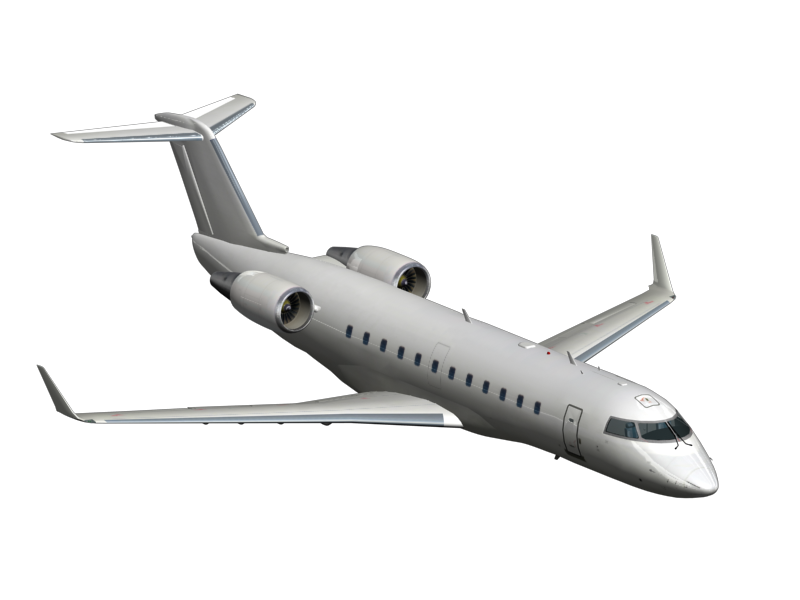
\includegraphics[width=\linewidth]{Figures/Bombardier_CRJ200}
  \end{minipage}%
  \begin{minipage}[b]{0.30\linewidth}
    \centering
    \begin{tabular}[b]{lll}
      \toprule
        \multicolumn{3}{c}{Legend} \\
      \midrule
        A & B & C \\
        0 & 0 & 0 \\
        0 & 1 & 0 \\
        1 & 0 & 0 \\
        1 & 1 & 1 \\
      \bottomrule
    \end{tabular}
    \vspace{5em}
  \end{minipage}
\caption{Figure and table side-by-side.}
\label{fig:side_by_side}
\end{figure}

 % file "Thesis_Results.tex"
\cleardoublepage

%%%%%%%%%%%%%%%%%%%%%%%%%%%%%%%%%%%%%%%%%%%%%%%%%%%%%%%%%%%%%%%%%%%%%%%%
%                                                                      %
%     File: Thesis_Conclusions.tex                                     %
%     Tex Master: Thesis.tex                                           %
%                                                                      %
%     Author: Andre C. Marta                                           %
%     Last modified :  2 Jul 2015                                      %
%                                                                      %
%%%%%%%%%%%%%%%%%%%%%%%%%%%%%%%%%%%%%%%%%%%%%%%%%%%%%%%%%%%%%%%%%%%%%%%%

\chapter{Conclusions}
\label{chapter:conclusions}

TO BE COMPLETED


% ----------------------------------------------------------------------
\section{Future Work}
\label{section:future}

TO BE COMPLETED
 % file "Thesis_Conclusions.tex"
\cleardoublepage

% ----------------------------------------------------------------------
%  Bibliography
% ----------------------------------------------------------------------

% Add entry in the table of contents as chapter
\phantomsection
\addcontentsline{toc}{chapter}{\bibname}

% Include all references in .bib file, even non-cited ones...
%\nocite{*} % this should be used carefully because it is not correct!

% Produces the bibliography section when processed by BibTeX
%
% Bibliography style
% > entries ordered alphabetically
%\bibliographystyle{plain}
% > unsorted with entries appearing in the order in which the citations appear.
%\bibliographystyle{unsrt}
% > entries ordered alphabetically, with first names and names of journals and months abbreviated
%\bibliographystyle{abbrv}
% > entries ordered alphabetically, with reference markers based on authors' initials and publication year
%\bibliographystyle{alpha}
%
% Replacement bibliography styles provided by 'natbib' package
% (plainnat.bst, abbrvnat.bst, unsrtnat.bst )
% > entries ordered alphabetically
%\bibliographystyle{plainnat}
% > unsorted with entries appearing in the order in which the citations appear.
%\bibliographystyle{unsrtnat}
% > entries ordered alphabetically, with first names and names of journals and months abbreviated
%\bibliographystyle{abbrvnat} % <<<<< SELECT IF USING REFERENCES BY AUTHOR/YEAR
% > entries ordered alphabetically, with reference markers based on authors' initials and publication year
%\bibliographystyle{alpha}
%
% Custom bibliography style adapted from 'natbib' package
%   (based on http://tex.stackexchange.com/questions/5053/is-it-possible-to-get-unsrt-abbrv-bibliography)
%   (unsrtnat.bst + abbrvnat.bst -> abbrvunsrtnat.bst)
%   (original files copied from:
%   http://tug.ctan.org/macros/latex/contrib/natbib/abbrvnat.bst
%   http://tug.ctan.org/macros/latex/contrib/natbib/unsrtnat.bst
% > unsorted with entries appearing in the order in which the citations appear, with first names and names of journals and months abbreviated.
\bibliographystyle{abbrvunsrtnat} % <<<<< SELECT IF USING REFERENCES BY NUMBER (CITATION ORDER)

% External bibliography database file in the BibTeX format
\bibliography{Thesis_bib_DB} % file "Thesis_bib_DB.bib"

\cleardoublepage

% ----------------------------------------------------------------------
%  Appendix (optional)
%
%  CAUTION: 1) the main document (up to the conclusions) shall not exceed 80 pages
%           2) the document shall not exceed a total of 100 pages (per IST regulations)
% ----------------------------------------------------------------------
\appendix

% add page number prefix according to apendix chapter (optional)
%\renewcommand{\thepage}{\thechapter.\arabic{page}}

% re-set arabic numbering (A.1,A.2,...) (optional, use only if chapter prefix is added)
%\setcounter{page}{1}

%%%%%%%%%%%%%%%%%%%%%%%%%%%%%%%%%%%%%%%%%%%%%%%%%%%%%%%%%%%%%%%%%%%%%%%%
%                                                                      %
%     File: Thesis_Appendix_A.tex                                      %
%     Tex Master: Thesis.tex                                           %
%                                                                      %
%     Author: Andre C. Marta                                           %
%     Last modified :  2 Jul 2015                                      %
%                                                                      %
%%%%%%%%%%%%%%%%%%%%%%%%%%%%%%%%%%%%%%%%%%%%%%%%%%%%%%%%%%%%%%%%%%%%%%%%

\chapter{Vector calculus}
\label{chapter:appendixVectors}

In case an appendix if deemed necessary, the document cannot exceed a total of 100 pages...

Some definitions and vector identities are listed in the section below.

% ----------------------------------------------------------------------
\section{Vector identities}
\label{section:vectorIdentities}

\begin{equation}
	\nabla \times \left( \nabla \phi \right) = 0
	\label{eq:cross_nnp}
\end{equation}

\begin{equation}
	\nabla \cdot \left( \nabla \times {\bf u} \right) = 0
	\label{eq:dotCross_nnu}
\end{equation}

 % file "Thesis_Appendix_A.tex"
\cleardoublepage

% re-set arabic numbering (B.1,B.2,...) (optional, use only if chapter prefix is added)
%\setcounter{page}{1}

%%%%%%%%%%%%%%%%%%%%%%%%%%%%%%%%%%%%%%%%%%%%%%%%%%%%%%%%%%%%%%%%%%%%%%%%
%                                                                      %
%     File: Thesis_Appendix_B.tex                                      %
%     Tex Master: Thesis.tex                                           %
%                                                                      %
%     Author: Andre C. Marta                                           %
%     Last modified :  2 Jul 2015                                      %
%                                                                      %
%%%%%%%%%%%%%%%%%%%%%%%%%%%%%%%%%%%%%%%%%%%%%%%%%%%%%%%%%%%%%%%%%%%%%%%%

\chapter{Technical Datasheets}
\label{chapter:appendixDatasheets}

It is possible to add PDF files to the document, such as technical sheets of some equipment used in the work.

% ----------------------------------------------------------------------
\section{Some Datasheet}
\label{section:datasheet}

% See more options to include PDF files in
% http://mirror.unl.edu/ctan/macros/latex/contrib/pdfpages/pdfpages.pdf
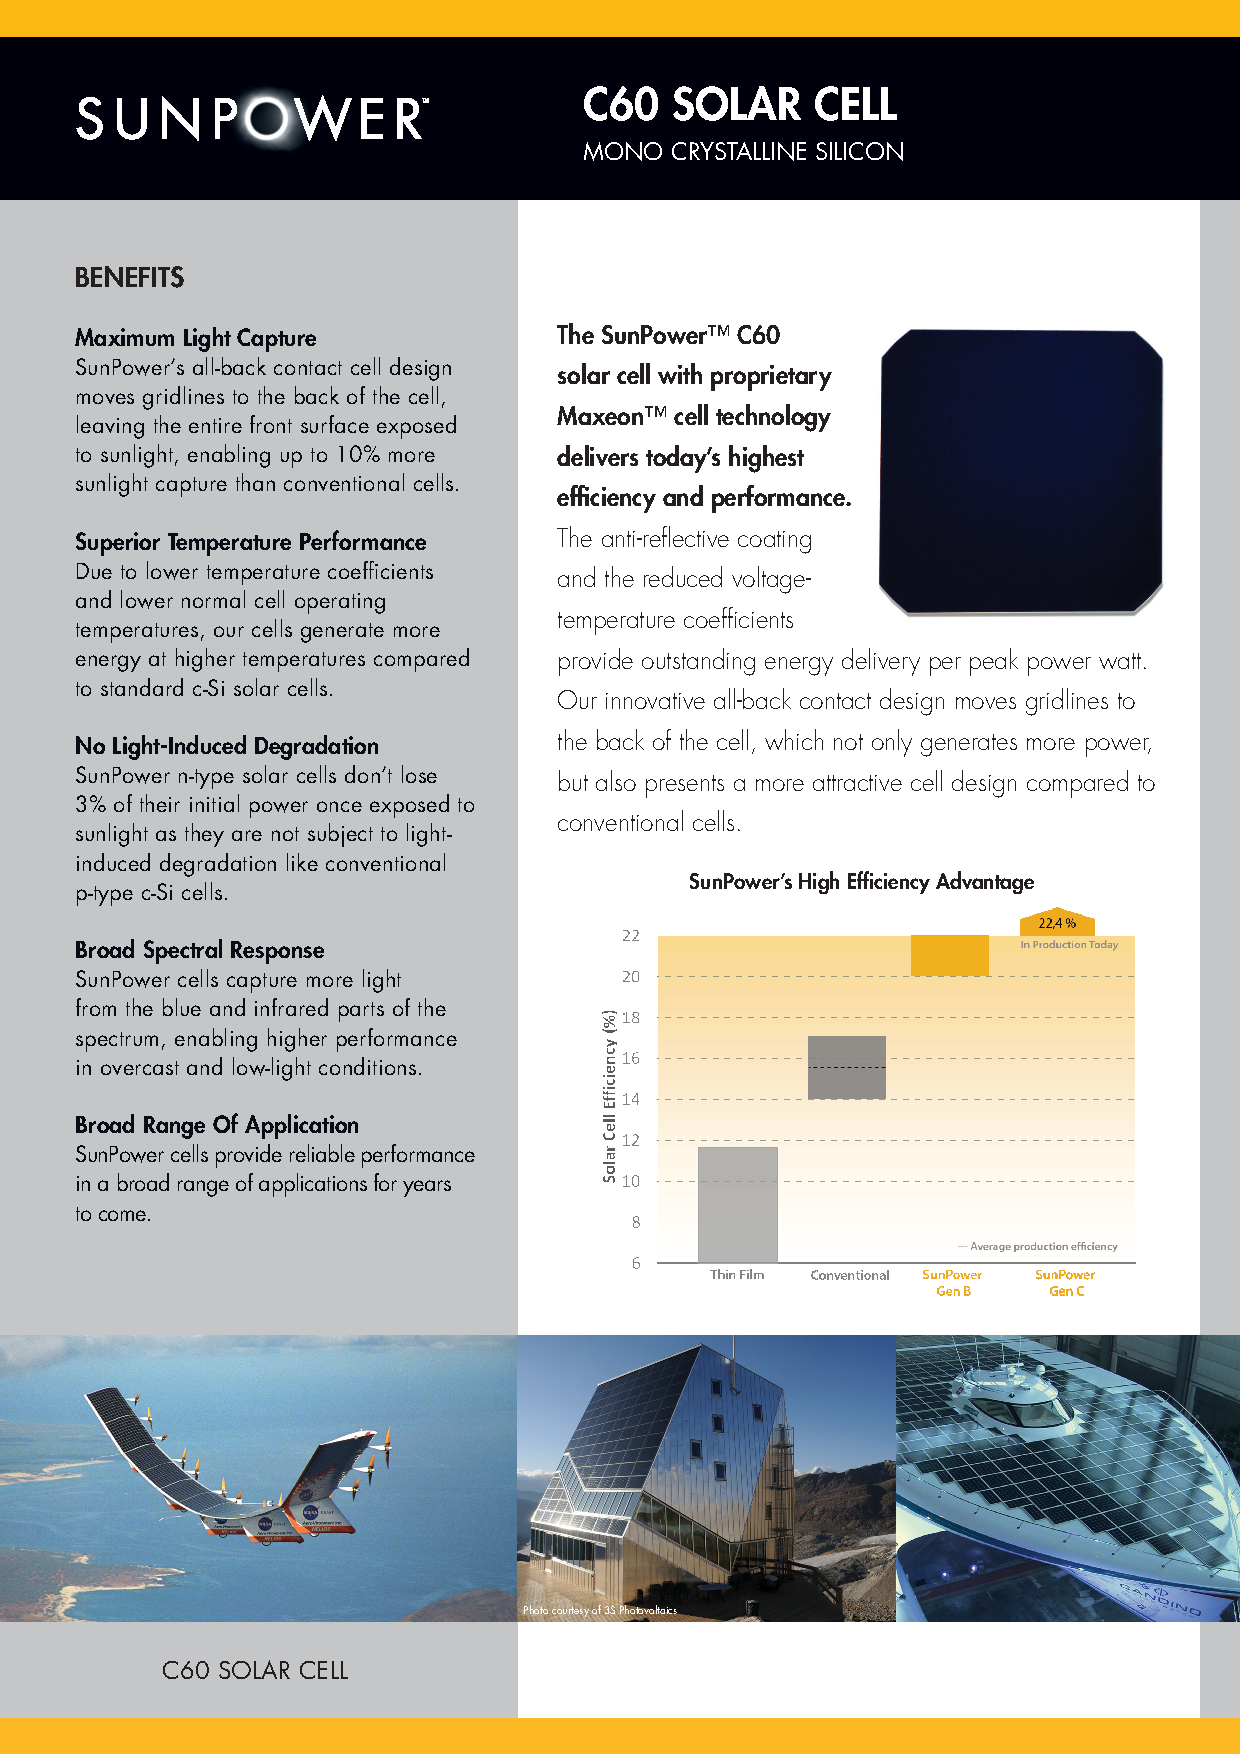
\includepdf[pages={1-2},nup=1x2,landscape=true]{Figures/SolarCell_Sunpower_C60.pdf}

 % file "Thesis_Appendix_B.tex"
\cleardoublepage

% ----------------------------------------------------------------------
\end{document}
% ----------------------------------------------------------------------
